% Options for packages loaded elsewhere
\PassOptionsToPackage{unicode}{hyperref}
\PassOptionsToPackage{hyphens}{url}
\PassOptionsToPackage{dvipsnames,svgnames,x11names}{xcolor}
%
\documentclass[
  letterpaper,
  DIV=11,
  numbers=noendperiod]{scrartcl}

\usepackage{amsmath,amssymb}
\usepackage{iftex}
\ifPDFTeX
  \usepackage[T1]{fontenc}
  \usepackage[utf8]{inputenc}
  \usepackage{textcomp} % provide euro and other symbols
\else % if luatex or xetex
  \usepackage{unicode-math}
  \defaultfontfeatures{Scale=MatchLowercase}
  \defaultfontfeatures[\rmfamily]{Ligatures=TeX,Scale=1}
\fi
\usepackage{lmodern}
\ifPDFTeX\else  
    % xetex/luatex font selection
\fi
% Use upquote if available, for straight quotes in verbatim environments
\IfFileExists{upquote.sty}{\usepackage{upquote}}{}
\IfFileExists{microtype.sty}{% use microtype if available
  \usepackage[]{microtype}
  \UseMicrotypeSet[protrusion]{basicmath} % disable protrusion for tt fonts
}{}
\makeatletter
\@ifundefined{KOMAClassName}{% if non-KOMA class
  \IfFileExists{parskip.sty}{%
    \usepackage{parskip}
  }{% else
    \setlength{\parindent}{0pt}
    \setlength{\parskip}{6pt plus 2pt minus 1pt}}
}{% if KOMA class
  \KOMAoptions{parskip=half}}
\makeatother
\usepackage{xcolor}
\setlength{\emergencystretch}{3em} % prevent overfull lines
\setcounter{secnumdepth}{-\maxdimen} % remove section numbering
% Make \paragraph and \subparagraph free-standing
\ifx\paragraph\undefined\else
  \let\oldparagraph\paragraph
  \renewcommand{\paragraph}[1]{\oldparagraph{#1}\mbox{}}
\fi
\ifx\subparagraph\undefined\else
  \let\oldsubparagraph\subparagraph
  \renewcommand{\subparagraph}[1]{\oldsubparagraph{#1}\mbox{}}
\fi

\usepackage{color}
\usepackage{fancyvrb}
\newcommand{\VerbBar}{|}
\newcommand{\VERB}{\Verb[commandchars=\\\{\}]}
\DefineVerbatimEnvironment{Highlighting}{Verbatim}{commandchars=\\\{\}}
% Add ',fontsize=\small' for more characters per line
\usepackage{framed}
\definecolor{shadecolor}{RGB}{241,243,245}
\newenvironment{Shaded}{\begin{snugshade}}{\end{snugshade}}
\newcommand{\AlertTok}[1]{\textcolor[rgb]{0.68,0.00,0.00}{#1}}
\newcommand{\AnnotationTok}[1]{\textcolor[rgb]{0.37,0.37,0.37}{#1}}
\newcommand{\AttributeTok}[1]{\textcolor[rgb]{0.40,0.45,0.13}{#1}}
\newcommand{\BaseNTok}[1]{\textcolor[rgb]{0.68,0.00,0.00}{#1}}
\newcommand{\BuiltInTok}[1]{\textcolor[rgb]{0.00,0.23,0.31}{#1}}
\newcommand{\CharTok}[1]{\textcolor[rgb]{0.13,0.47,0.30}{#1}}
\newcommand{\CommentTok}[1]{\textcolor[rgb]{0.37,0.37,0.37}{#1}}
\newcommand{\CommentVarTok}[1]{\textcolor[rgb]{0.37,0.37,0.37}{\textit{#1}}}
\newcommand{\ConstantTok}[1]{\textcolor[rgb]{0.56,0.35,0.01}{#1}}
\newcommand{\ControlFlowTok}[1]{\textcolor[rgb]{0.00,0.23,0.31}{#1}}
\newcommand{\DataTypeTok}[1]{\textcolor[rgb]{0.68,0.00,0.00}{#1}}
\newcommand{\DecValTok}[1]{\textcolor[rgb]{0.68,0.00,0.00}{#1}}
\newcommand{\DocumentationTok}[1]{\textcolor[rgb]{0.37,0.37,0.37}{\textit{#1}}}
\newcommand{\ErrorTok}[1]{\textcolor[rgb]{0.68,0.00,0.00}{#1}}
\newcommand{\ExtensionTok}[1]{\textcolor[rgb]{0.00,0.23,0.31}{#1}}
\newcommand{\FloatTok}[1]{\textcolor[rgb]{0.68,0.00,0.00}{#1}}
\newcommand{\FunctionTok}[1]{\textcolor[rgb]{0.28,0.35,0.67}{#1}}
\newcommand{\ImportTok}[1]{\textcolor[rgb]{0.00,0.46,0.62}{#1}}
\newcommand{\InformationTok}[1]{\textcolor[rgb]{0.37,0.37,0.37}{#1}}
\newcommand{\KeywordTok}[1]{\textcolor[rgb]{0.00,0.23,0.31}{#1}}
\newcommand{\NormalTok}[1]{\textcolor[rgb]{0.00,0.23,0.31}{#1}}
\newcommand{\OperatorTok}[1]{\textcolor[rgb]{0.37,0.37,0.37}{#1}}
\newcommand{\OtherTok}[1]{\textcolor[rgb]{0.00,0.23,0.31}{#1}}
\newcommand{\PreprocessorTok}[1]{\textcolor[rgb]{0.68,0.00,0.00}{#1}}
\newcommand{\RegionMarkerTok}[1]{\textcolor[rgb]{0.00,0.23,0.31}{#1}}
\newcommand{\SpecialCharTok}[1]{\textcolor[rgb]{0.37,0.37,0.37}{#1}}
\newcommand{\SpecialStringTok}[1]{\textcolor[rgb]{0.13,0.47,0.30}{#1}}
\newcommand{\StringTok}[1]{\textcolor[rgb]{0.13,0.47,0.30}{#1}}
\newcommand{\VariableTok}[1]{\textcolor[rgb]{0.07,0.07,0.07}{#1}}
\newcommand{\VerbatimStringTok}[1]{\textcolor[rgb]{0.13,0.47,0.30}{#1}}
\newcommand{\WarningTok}[1]{\textcolor[rgb]{0.37,0.37,0.37}{\textit{#1}}}

\providecommand{\tightlist}{%
  \setlength{\itemsep}{0pt}\setlength{\parskip}{0pt}}\usepackage{longtable,booktabs,array}
\usepackage{calc} % for calculating minipage widths
% Correct order of tables after \paragraph or \subparagraph
\usepackage{etoolbox}
\makeatletter
\patchcmd\longtable{\par}{\if@noskipsec\mbox{}\fi\par}{}{}
\makeatother
% Allow footnotes in longtable head/foot
\IfFileExists{footnotehyper.sty}{\usepackage{footnotehyper}}{\usepackage{footnote}}
\makesavenoteenv{longtable}
\usepackage{graphicx}
\makeatletter
\def\maxwidth{\ifdim\Gin@nat@width>\linewidth\linewidth\else\Gin@nat@width\fi}
\def\maxheight{\ifdim\Gin@nat@height>\textheight\textheight\else\Gin@nat@height\fi}
\makeatother
% Scale images if necessary, so that they will not overflow the page
% margins by default, and it is still possible to overwrite the defaults
% using explicit options in \includegraphics[width, height, ...]{}
\setkeys{Gin}{width=\maxwidth,height=\maxheight,keepaspectratio}
% Set default figure placement to htbp
\makeatletter
\def\fps@figure{htbp}
\makeatother

\KOMAoption{captions}{tableheading}
\makeatletter
\makeatother
\makeatletter
\makeatother
\makeatletter
\@ifpackageloaded{caption}{}{\usepackage{caption}}
\AtBeginDocument{%
\ifdefined\contentsname
  \renewcommand*\contentsname{Table of contents}
\else
  \newcommand\contentsname{Table of contents}
\fi
\ifdefined\listfigurename
  \renewcommand*\listfigurename{List of Figures}
\else
  \newcommand\listfigurename{List of Figures}
\fi
\ifdefined\listtablename
  \renewcommand*\listtablename{List of Tables}
\else
  \newcommand\listtablename{List of Tables}
\fi
\ifdefined\figurename
  \renewcommand*\figurename{Figure}
\else
  \newcommand\figurename{Figure}
\fi
\ifdefined\tablename
  \renewcommand*\tablename{Table}
\else
  \newcommand\tablename{Table}
\fi
}
\@ifpackageloaded{float}{}{\usepackage{float}}
\floatstyle{ruled}
\@ifundefined{c@chapter}{\newfloat{codelisting}{h}{lop}}{\newfloat{codelisting}{h}{lop}[chapter]}
\floatname{codelisting}{Listing}
\newcommand*\listoflistings{\listof{codelisting}{List of Listings}}
\makeatother
\makeatletter
\@ifpackageloaded{caption}{}{\usepackage{caption}}
\@ifpackageloaded{subcaption}{}{\usepackage{subcaption}}
\makeatother
\makeatletter
\@ifpackageloaded{tcolorbox}{}{\usepackage[skins,breakable]{tcolorbox}}
\makeatother
\makeatletter
\@ifundefined{shadecolor}{\definecolor{shadecolor}{rgb}{.97, .97, .97}}
\makeatother
\makeatletter
\makeatother
\makeatletter
\makeatother
\ifLuaTeX
  \usepackage{selnolig}  % disable illegal ligatures
\fi
\IfFileExists{bookmark.sty}{\usepackage{bookmark}}{\usepackage{hyperref}}
\IfFileExists{xurl.sty}{\usepackage{xurl}}{} % add URL line breaks if available
\urlstyle{same} % disable monospaced font for URLs
\hypersetup{
  pdftitle={Universidades},
  pdfauthor={Joaquin Bermejo, Franco Scarafia y Gerard Seward},
  colorlinks=true,
  linkcolor={blue},
  filecolor={Maroon},
  citecolor={Blue},
  urlcolor={Blue},
  pdfcreator={LaTeX via pandoc}}

\title{Universidades}
\usepackage{etoolbox}
\makeatletter
\providecommand{\subtitle}[1]{% add subtitle to \maketitle
  \apptocmd{\@title}{\par {\large #1 \par}}{}{}
}
\makeatother
\subtitle{TP Final - Regresion avanzada}
\author{Joaquin Bermejo, Franco Scarafia y Gerard Seward}
\date{}

\begin{document}
\maketitle
\ifdefined\Shaded\renewenvironment{Shaded}{\begin{tcolorbox}[borderline west={3pt}{0pt}{shadecolor}, interior hidden, breakable, enhanced, boxrule=0pt, sharp corners, frame hidden]}{\end{tcolorbox}}\fi

\hypertarget{introduccion}{%
\section{Introduccion}\label{introduccion}}

Se nos presenta una base de datos sobre universidades publicas y
privadas con las siguientes variables

\begin{longtable}[]{@{}
  >{\raggedright\arraybackslash}p{(\columnwidth - 2\tabcolsep) * \real{0.3380}}
  >{\raggedright\arraybackslash}p{(\columnwidth - 2\tabcolsep) * \real{0.6620}}@{}}
\toprule\noalign{}
\begin{minipage}[b]{\linewidth}\raggedright
Variable
\end{minipage} & \begin{minipage}[b]{\linewidth}\raggedright
Descripción
\end{minipage} \\
\midrule\noalign{}
\endhead
\bottomrule\noalign{}
\endlastfoot
\texttt{privada} & indica si la universidad es privada o no. \\
\texttt{aplicaciones} & cantidad de aplicaciones recibidas por la
universidad durante el último año (cada estudiante que aspira a ingresar
debe presentar una aplicación formal, a partir de la cual es admitido/a
o rechazado/a), medida en miles de personas. \\
\texttt{ingresantes} & cantidad de aplicaciones aceptadas, medida en
miles de personas. \\
\texttt{estudiantes} & cantidad total de estudiantes en carreras de
grado, medida en miles de personas. \\
\texttt{top10} & porcentaje de ingresantes que fueron parte del 10\% de
estudiantes con mejores calificaciones en sus respectivas escuelas
secundarias. \\
\texttt{cuota} & costo de la cuota de la universidad, medida en miles de
dólares. \\
\texttt{prof\_dr} & porcentaje de profesores de la universidad que
poseen título de doctorado. \\
\texttt{razon} & tasa de estudiantes por profesor. \\
\texttt{tasa\_grad} & porcentaje de estudiantes que se gradúan. \\
\end{longtable}

La variable de interés es \texttt{tasa\_grad} que indica el porcentaje
de estudiantes que se gradúan

A continuacion se importan las librerias que utilizaremos y se lee la
funte de la base de datos

\begin{Shaded}
\begin{Highlighting}[]
\FunctionTok{library}\NormalTok{(tidyverse)}
\FunctionTok{library}\NormalTok{(ggplot2)}
\FunctionTok{library}\NormalTok{(MASS)}
\FunctionTok{library}\NormalTok{(GGally)}
\FunctionTok{library}\NormalTok{(caret)}
\end{Highlighting}
\end{Shaded}

\begin{verbatim}
Warning: package 'caret' was built under R version 4.3.2
\end{verbatim}

\begin{Shaded}
\begin{Highlighting}[]
\FunctionTok{library}\NormalTok{(corrplot)}
\end{Highlighting}
\end{Shaded}

\begin{verbatim}
Warning: package 'corrplot' was built under R version 4.3.2
\end{verbatim}

\begin{Shaded}
\begin{Highlighting}[]
\FunctionTok{library}\NormalTok{(janitor)}
\FunctionTok{library}\NormalTok{(knitr)}
\FunctionTok{library}\NormalTok{(leaps)}
\FunctionTok{library}\NormalTok{(pROC)}
\end{Highlighting}
\end{Shaded}

\begin{verbatim}
Warning: package 'pROC' was built under R version 4.3.2
\end{verbatim}

\begin{Shaded}
\begin{Highlighting}[]
\FunctionTok{library}\NormalTok{(glmnet)}
\end{Highlighting}
\end{Shaded}

\begin{verbatim}
Warning: package 'glmnet' was built under R version 4.3.3
\end{verbatim}

\begin{Shaded}
\begin{Highlighting}[]
\NormalTok{df }\OtherTok{=} \FunctionTok{read.delim}\NormalTok{(}\StringTok{\textquotesingle{}1{-}data/universidades.txt\textquotesingle{}}\NormalTok{)}
\NormalTok{df }\OtherTok{=}\NormalTok{ df }\SpecialCharTok{\%\textgreater{}\%} 
  \FunctionTok{mutate}\NormalTok{(}\AttributeTok{privada =} \FunctionTok{ifelse}\NormalTok{(privada }\SpecialCharTok{==} \StringTok{"Si"}\NormalTok{, }\ConstantTok{TRUE}\NormalTok{, }\ConstantTok{FALSE}\NormalTok{))}

\CommentTok{\# categoricals\_vars \textless{}{-} df \%\textgreater{}\%}
\CommentTok{\#   select(where(is.factor)) \%\textgreater{}\%}
\CommentTok{\#   names()}

\CommentTok{\# continuous\_vars \textless{}{-} df \%\textgreater{}\%}
\CommentTok{\#   select(where(is.numeric)) \%\textgreater{}\%}
\CommentTok{\#   names()}
\end{Highlighting}
\end{Shaded}

Estos son los primeros 5 registro para entender como estan representados
los datos

\begin{Shaded}
\begin{Highlighting}[]
\FunctionTok{head}\NormalTok{(df)}
\end{Highlighting}
\end{Shaded}

\begin{verbatim}
  privada aplicaciones ingresantes estudiantes top10 cuota prof_dr razon
1    TRUE        1.660       0.721       2.885    23  7.44      70  18.1
2    TRUE        2.186       0.512       2.683    16 12.28      29  12.2
3    TRUE        1.428       0.336       1.036    22 11.25      53  12.9
4    TRUE        0.417       0.137       0.510    60 12.96      92   7.7
5    TRUE        0.193       0.055       0.249    16  7.56      76  11.9
6    TRUE        0.587       0.158       0.678    38 13.50      67   9.4
  tasa_grad
1        60
2        56
3        54
4        59
5        15
6        55
\end{verbatim}

\hypertarget{resumen-de-los-datos}{%
\section{Resumen de los datos}\label{resumen-de-los-datos}}

\begin{Shaded}
\begin{Highlighting}[]
\NormalTok{skimr}\SpecialCharTok{::}\FunctionTok{skim}\NormalTok{(df)}
\end{Highlighting}
\end{Shaded}

\begin{longtable}[]{@{}ll@{}}
\caption{Data summary}\tabularnewline
\toprule\noalign{}
\endfirsthead
\endhead
\bottomrule\noalign{}
\endlastfoot
Name & df \\
Number of rows & 777 \\
Number of columns & 9 \\
\_\_\_\_\_\_\_\_\_\_\_\_\_\_\_\_\_\_\_\_\_\_\_ & \\
Column type frequency: & \\
logical & 1 \\
numeric & 8 \\
\_\_\_\_\_\_\_\_\_\_\_\_\_\_\_\_\_\_\_\_\_\_\_\_ & \\
Group variables & None \\
\end{longtable}

\textbf{Variable type: logical}

\begin{longtable}[]{@{}lrrrl@{}}
\toprule\noalign{}
skim\_variable & n\_missing & complete\_rate & mean & count \\
\midrule\noalign{}
\endhead
\bottomrule\noalign{}
\endlastfoot
privada & 0 & 1 & 0.73 & TRU: 565, FAL: 212 \\
\end{longtable}

\textbf{Variable type: numeric}

\begin{longtable}[]{@{}
  >{\raggedright\arraybackslash}p{(\columnwidth - 20\tabcolsep) * \real{0.1609}}
  >{\raggedleft\arraybackslash}p{(\columnwidth - 20\tabcolsep) * \real{0.1149}}
  >{\raggedleft\arraybackslash}p{(\columnwidth - 20\tabcolsep) * \real{0.1609}}
  >{\raggedleft\arraybackslash}p{(\columnwidth - 20\tabcolsep) * \real{0.0690}}
  >{\raggedleft\arraybackslash}p{(\columnwidth - 20\tabcolsep) * \real{0.0690}}
  >{\raggedleft\arraybackslash}p{(\columnwidth - 20\tabcolsep) * \real{0.0690}}
  >{\raggedleft\arraybackslash}p{(\columnwidth - 20\tabcolsep) * \real{0.0690}}
  >{\raggedleft\arraybackslash}p{(\columnwidth - 20\tabcolsep) * \real{0.0690}}
  >{\raggedleft\arraybackslash}p{(\columnwidth - 20\tabcolsep) * \real{0.0690}}
  >{\raggedleft\arraybackslash}p{(\columnwidth - 20\tabcolsep) * \real{0.0805}}
  >{\raggedright\arraybackslash}p{(\columnwidth - 20\tabcolsep) * \real{0.0690}}@{}}
\toprule\noalign{}
\begin{minipage}[b]{\linewidth}\raggedright
skim\_variable
\end{minipage} & \begin{minipage}[b]{\linewidth}\raggedleft
n\_missing
\end{minipage} & \begin{minipage}[b]{\linewidth}\raggedleft
complete\_rate
\end{minipage} & \begin{minipage}[b]{\linewidth}\raggedleft
mean
\end{minipage} & \begin{minipage}[b]{\linewidth}\raggedleft
sd
\end{minipage} & \begin{minipage}[b]{\linewidth}\raggedleft
p0
\end{minipage} & \begin{minipage}[b]{\linewidth}\raggedleft
p25
\end{minipage} & \begin{minipage}[b]{\linewidth}\raggedleft
p50
\end{minipage} & \begin{minipage}[b]{\linewidth}\raggedleft
p75
\end{minipage} & \begin{minipage}[b]{\linewidth}\raggedleft
p100
\end{minipage} & \begin{minipage}[b]{\linewidth}\raggedright
hist
\end{minipage} \\
\midrule\noalign{}
\endhead
\bottomrule\noalign{}
\endlastfoot
aplicaciones & 0 & 1 & 3.00 & 3.87 & 0.08 & 0.78 & 1.56 & 3.62 & 48.09 &
▇▁▁▁▁ \\
ingresantes & 0 & 1 & 0.78 & 0.93 & 0.04 & 0.24 & 0.43 & 0.90 & 6.39 &
▇▁▁▁▁ \\
estudiantes & 0 & 1 & 3.70 & 4.85 & 0.14 & 0.99 & 1.71 & 4.00 & 31.64 &
▇▁▁▁▁ \\
top10 & 0 & 1 & 27.56 & 17.64 & 1.00 & 15.00 & 23.00 & 35.00 & 96.00 &
▇▇▂▁▁ \\
cuota & 0 & 1 & 10.44 & 4.02 & 2.34 & 7.32 & 9.99 & 12.93 & 21.70 &
▃▇▆▂▂ \\
prof\_dr & 0 & 1 & 72.66 & 16.32 & 8.00 & 62.00 & 75.00 & 85.00 & 100.00
& ▁▁▅▇▇ \\
razon & 0 & 1 & 14.09 & 3.96 & 2.50 & 11.50 & 13.60 & 16.50 & 39.80 &
▁▇▂▁▁ \\
tasa\_grad & 0 & 1 & 65.44 & 17.12 & 10.00 & 53.00 & 65.00 & 78.00 &
100.00 & ▁▂▇▇▅ \\
\end{longtable}

\begin{Shaded}
\begin{Highlighting}[]
\FunctionTok{corrplot}\NormalTok{(}\FunctionTok{cor}\NormalTok{(dplyr}\SpecialCharTok{::}\FunctionTok{select}\NormalTok{(df, }\SpecialCharTok{{-}}\NormalTok{privada)),}
         \AttributeTok{method =} \StringTok{"color"}\NormalTok{,}
         \AttributeTok{type =} \StringTok{"lower"}\NormalTok{, }
         \AttributeTok{addCoef.col =} \StringTok{"black"}\NormalTok{,}
         \AttributeTok{tl.cex =} \FloatTok{0.6}\NormalTok{,}
         \AttributeTok{tl.pos =} \StringTok{"ld"}\NormalTok{,}
         \AttributeTok{tl.srt =} \DecValTok{45}\NormalTok{,}
         \AttributeTok{title =} \StringTok{"Correlation Plot for Numerical Variables"}\NormalTok{,}
         \AttributeTok{order =} \StringTok{"hclust"}\NormalTok{,}
         \AttributeTok{mar =} \FunctionTok{c}\NormalTok{(}\DecValTok{0}\NormalTok{, }\DecValTok{0}\NormalTok{, }\DecValTok{2}\NormalTok{, }\DecValTok{0}\NormalTok{))}
\end{Highlighting}
\end{Shaded}

\begin{figure}[H]

{\centering 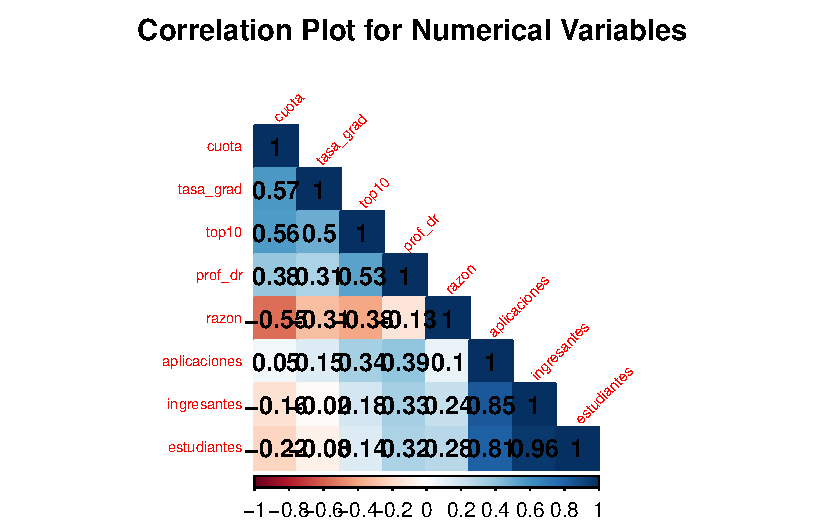
\includegraphics{TP_final_files/figure-pdf/unnamed-chunk-4-1.pdf}

}

\end{figure}

\begin{Shaded}
\begin{Highlighting}[]
\CommentTok{\#ggpairs(df)}
\CommentTok{\#ggpairs(df, aes(colour = privada, alpha = 0.4))}
\end{Highlighting}
\end{Shaded}

Para la variable target \texttt{tasa\_grad}, los coeficientes de pearson
mas relevantes se dan para la siguientes variables,

\begin{enumerate}
\def\labelenumi{\arabic{enumi}.}
\tightlist
\item
  \texttt{cuota} con un valor positivo de 0.57
\item
  \texttt{top10} con un valor positivo de 0.5
\item
  \texttt{prof\_dr} con un valor positivo de 0.31
\item
  \texttt{razon} con un valor negativo de 0.31
\end{enumerate}

\hypertarget{privada}{%
\subsection{Privada}\label{privada}}

\begin{Shaded}
\begin{Highlighting}[]
\FunctionTok{ggplot}\NormalTok{(df, }\FunctionTok{aes}\NormalTok{(}\AttributeTok{x =}\NormalTok{ privada, }\AttributeTok{fill =}\NormalTok{ privada))}\SpecialCharTok{+}
  \FunctionTok{geom\_bar}\NormalTok{() }\SpecialCharTok{+} 
  \FunctionTok{labs}\NormalTok{(}\AttributeTok{title =} \StringTok{"Cantidad de alumnos por tipo de universidad"}\NormalTok{,}
       \AttributeTok{x =} \StringTok{"Tipo"}\NormalTok{,}
       \AttributeTok{y =} \StringTok{"Cant. alumnos"}\NormalTok{)}\SpecialCharTok{+}
  \FunctionTok{theme\_minimal}\NormalTok{()}
\end{Highlighting}
\end{Shaded}

\begin{figure}[H]

{\centering 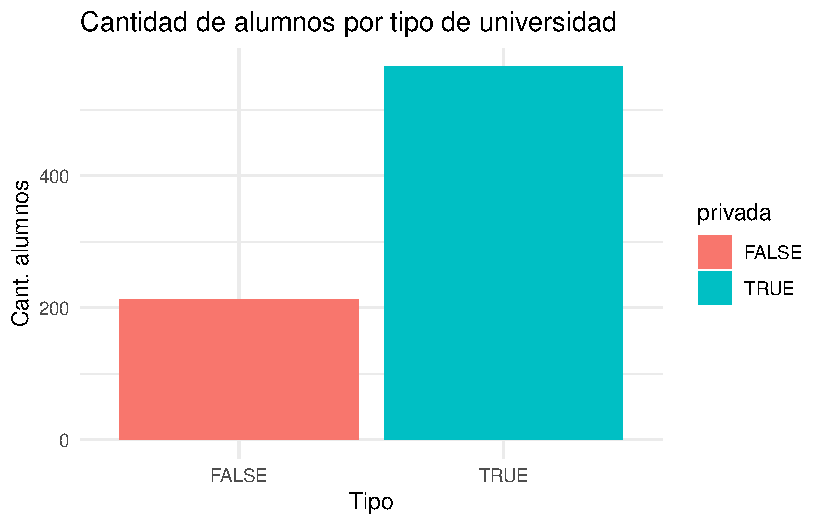
\includegraphics{TP_final_files/figure-pdf/unnamed-chunk-5-1.pdf}

}

\end{figure}

\begin{Shaded}
\begin{Highlighting}[]
\FunctionTok{ggplot}\NormalTok{(df) }\SpecialCharTok{+}
  \FunctionTok{aes}\NormalTok{(}\AttributeTok{x =}\NormalTok{ tasa\_grad) }\SpecialCharTok{+} 
  \FunctionTok{geom\_histogram}\NormalTok{(}\AttributeTok{na.rm =} \ConstantTok{TRUE}\NormalTok{, }\AttributeTok{bins =} \DecValTok{12}\NormalTok{, }\AttributeTok{color =} \StringTok{"black"}\NormalTok{, }\FunctionTok{aes}\NormalTok{(}\AttributeTok{fill =}\NormalTok{ privada)) }\SpecialCharTok{+} 
  \FunctionTok{facet\_wrap}\NormalTok{(}\SpecialCharTok{\textasciitilde{}}\NormalTok{ privada) }\SpecialCharTok{+} 
  \FunctionTok{theme}\NormalTok{(}\AttributeTok{legend.position =} \StringTok{"bottom"}\NormalTok{)}\SpecialCharTok{+}
  \FunctionTok{theme\_minimal}\NormalTok{()}
\end{Highlighting}
\end{Shaded}

\begin{figure}[H]

{\centering 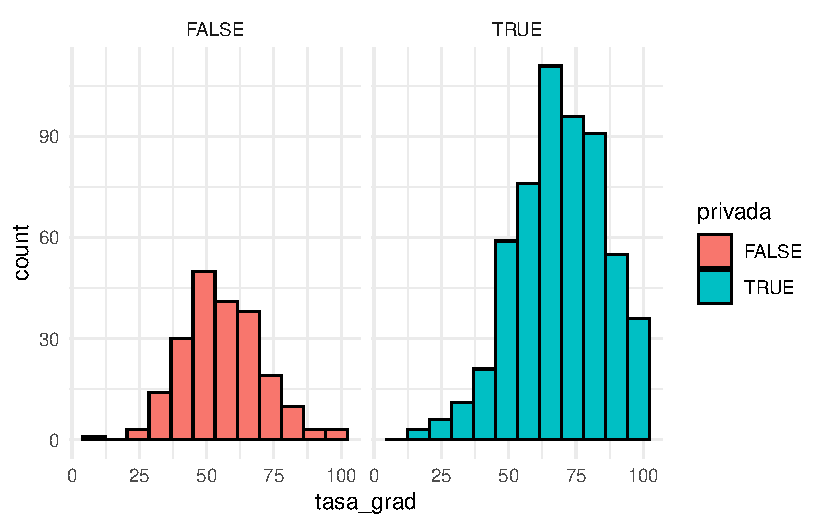
\includegraphics{TP_final_files/figure-pdf/unnamed-chunk-6-1.pdf}

}

\end{figure}

La variable \texttt{privada} es de tipo categórica con valores positivos
(565) y negativos (212) cuya tasa de graduados se comporta diferente.
Las universidades privadas tienden a tener una mayor tasa de graduados

\hypertarget{cuota}{%
\subsection{Cuota}\label{cuota}}

\begin{Shaded}
\begin{Highlighting}[]
\FunctionTok{ggplot}\NormalTok{(df, }\FunctionTok{aes}\NormalTok{(cuota))}\SpecialCharTok{+}
  \FunctionTok{geom\_histogram}\NormalTok{(}\AttributeTok{bins =} \DecValTok{30}\NormalTok{, }\FunctionTok{aes}\NormalTok{(}\AttributeTok{fill =} \StringTok{"\#F8766D"}\NormalTok{, }\AttributeTok{y =} \FunctionTok{after\_stat}\NormalTok{(density)))}\SpecialCharTok{+}
  \FunctionTok{geom\_density}\NormalTok{(}\AttributeTok{color =} \StringTok{"blue"}\NormalTok{)}\SpecialCharTok{+}
  \FunctionTok{labs}\NormalTok{(}\AttributeTok{title =} \StringTok{"Histograma de cuota"}\NormalTok{,}
       \AttributeTok{x =} \StringTok{"Cuota"}\NormalTok{)}\SpecialCharTok{+}
  \FunctionTok{theme\_minimal}\NormalTok{()}\SpecialCharTok{+}
  \FunctionTok{theme}\NormalTok{(}\AttributeTok{legend.position =} \StringTok{"none"}\NormalTok{)}
\end{Highlighting}
\end{Shaded}

\begin{figure}[H]

{\centering 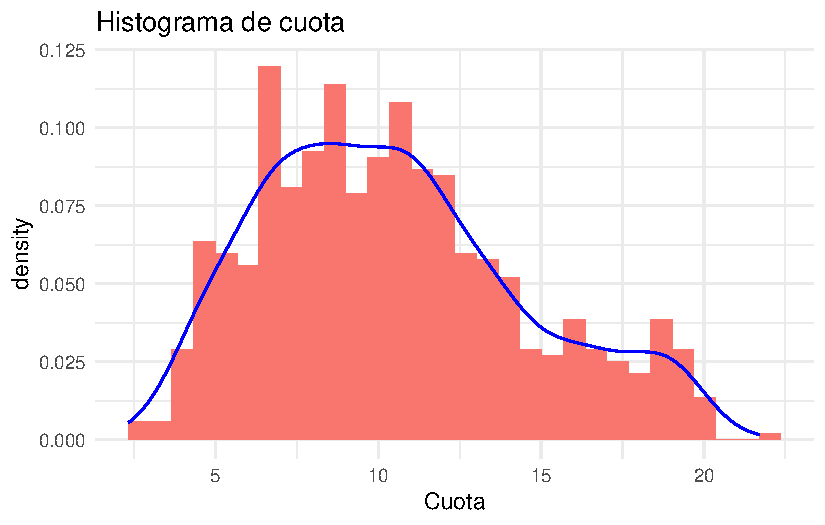
\includegraphics{TP_final_files/figure-pdf/unnamed-chunk-7-1.pdf}

}

\end{figure}

\begin{Shaded}
\begin{Highlighting}[]
\FunctionTok{ggplot}\NormalTok{(df, }\FunctionTok{aes}\NormalTok{(}\AttributeTok{x =}\NormalTok{ cuota, }\AttributeTok{y =}\NormalTok{ tasa\_grad, }\AttributeTok{color =}\NormalTok{ privada)) }\SpecialCharTok{+}
  \FunctionTok{geom\_point}\NormalTok{() }\SpecialCharTok{+} 
  \FunctionTok{geom\_smooth}\NormalTok{(}\AttributeTok{formula =} \StringTok{"y \textasciitilde{} x"}\NormalTok{, }\AttributeTok{method =} \StringTok{"lm"}\NormalTok{, }\AttributeTok{se =} \ConstantTok{FALSE}\NormalTok{)}\SpecialCharTok{+}
  \FunctionTok{labs}\NormalTok{(}\AttributeTok{title =} \StringTok{"Cuota vs Tasa de graduados"}\NormalTok{,}
       \AttributeTok{x =} \StringTok{"Cuota"}\NormalTok{,}
       \AttributeTok{y =} \StringTok{"\% de graduados"}\NormalTok{)}\SpecialCharTok{+}
  \FunctionTok{theme\_minimal}\NormalTok{()}
\end{Highlighting}
\end{Shaded}

\begin{figure}[H]

{\centering 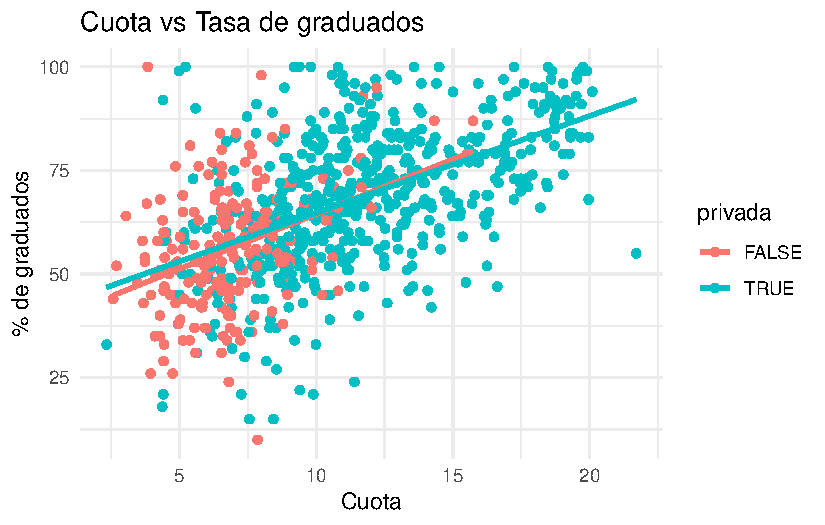
\includegraphics{TP_final_files/figure-pdf/unnamed-chunk-8-1.pdf}

}

\end{figure}

La variable \texttt{cuota} es de tipo cuantitativa con las siguientes
métricas estadísticas

\begin{longtable}[]{@{}ll@{}}
\toprule\noalign{}
Variable & Valor \\
\midrule\noalign{}
\endhead
\bottomrule\noalign{}
\endlastfoot
Maximo & \texttt{\{r\}\ round(max(df\$cuota),2)} \\
Promedio & \texttt{\{r\}\ round(mean(df\$cuota),2)} \\
Minimo & \texttt{\{r\}\ round(min(df\$cuota),2)} \\
Desviacion & \texttt{\{r\}\ round(sd(df\$cuota),2)} \\
\end{longtable}

Al graficar esta variable con el target notamos una relación lineal,
aunque con mucha dispersión, donde para valores bajos de cuota hay una
mayor variación entre el valor real con el un valor predicho con una
regresión lineal donde \texttt{tasa\_grad} \textasciitilde{}
\texttt{cuota}

\hypertarget{aplicaciones}{%
\subsection{Aplicaciones}\label{aplicaciones}}

\begin{Shaded}
\begin{Highlighting}[]
\FunctionTok{ggplot}\NormalTok{(df, }\FunctionTok{aes}\NormalTok{(aplicaciones))}\SpecialCharTok{+}
  \FunctionTok{geom\_histogram}\NormalTok{(}\AttributeTok{bins =} \DecValTok{30}\NormalTok{, }\FunctionTok{aes}\NormalTok{(}\AttributeTok{fill =} \StringTok{"\#F8766D"}\NormalTok{, }\AttributeTok{y =} \FunctionTok{after\_stat}\NormalTok{(density)))}\SpecialCharTok{+}
  \FunctionTok{geom\_density}\NormalTok{(}\AttributeTok{color =} \StringTok{"blue"}\NormalTok{)}\SpecialCharTok{+}
  \FunctionTok{labs}\NormalTok{(}\AttributeTok{title =} \StringTok{"Histograma de aplicaciones"}\NormalTok{,}
       \AttributeTok{x =} \StringTok{"aplicaciones"}\NormalTok{)}\SpecialCharTok{+}
  \FunctionTok{theme\_minimal}\NormalTok{()}\SpecialCharTok{+}
  \FunctionTok{theme}\NormalTok{(}\AttributeTok{legend.position =} \StringTok{"none"}\NormalTok{)}
\end{Highlighting}
\end{Shaded}

\begin{figure}[H]

{\centering 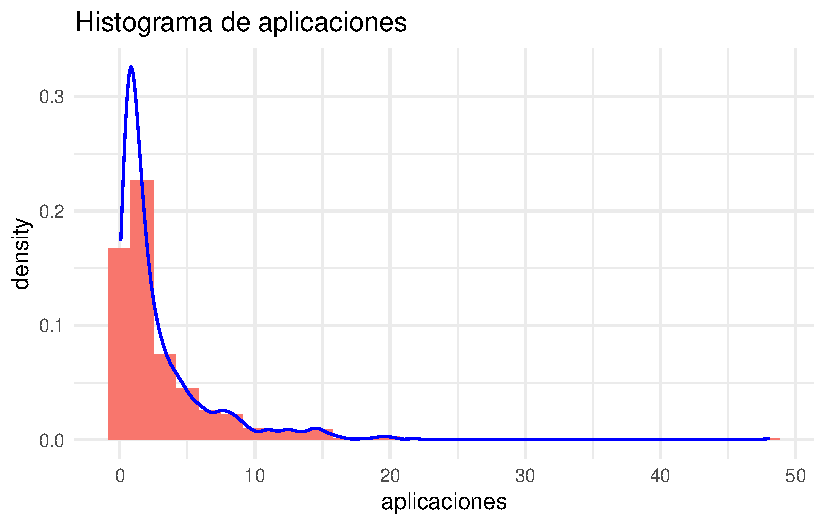
\includegraphics{TP_final_files/figure-pdf/unnamed-chunk-9-1.pdf}

}

\end{figure}

\begin{Shaded}
\begin{Highlighting}[]
\FunctionTok{ggplot}\NormalTok{(df, }\FunctionTok{aes}\NormalTok{(}\AttributeTok{x =}\NormalTok{ aplicaciones, }\AttributeTok{y =}\NormalTok{ tasa\_grad, }\AttributeTok{color =}\NormalTok{ privada)) }\SpecialCharTok{+}
  \FunctionTok{geom\_point}\NormalTok{() }\SpecialCharTok{+} 
  \FunctionTok{geom\_smooth}\NormalTok{(}\AttributeTok{formula =} \StringTok{"y \textasciitilde{} x"}\NormalTok{, }\AttributeTok{method =} \StringTok{"lm"}\NormalTok{, }\AttributeTok{se =} \ConstantTok{FALSE}\NormalTok{)}\SpecialCharTok{+}
  \FunctionTok{labs}\NormalTok{(}\AttributeTok{title =} \StringTok{"aplicaciones vs Tasa de graduados"}\NormalTok{,}
       \AttributeTok{x =} \StringTok{"aplicaciones"}\NormalTok{,}
       \AttributeTok{y =} \StringTok{"\% de graduados"}\NormalTok{)}\SpecialCharTok{+}
  \FunctionTok{theme\_minimal}\NormalTok{()}
\end{Highlighting}
\end{Shaded}

\begin{figure}[H]

{\centering 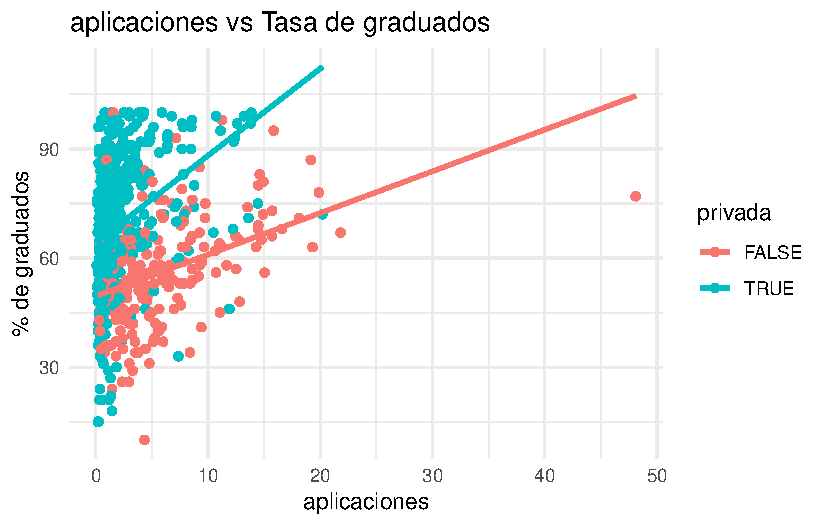
\includegraphics{TP_final_files/figure-pdf/unnamed-chunk-10-1.pdf}

}

\end{figure}

La variable \texttt{aplicaciones} es de tipo cuantitativa donde hay una
concentración de observaciones grandes para valores bajos de
aplicaciones.

No se observa una clara relación lineal contra \texttt{tasa\_grad}

\hypertarget{ingresantes}{%
\subsection{Ingresantes}\label{ingresantes}}

\begin{Shaded}
\begin{Highlighting}[]
\FunctionTok{ggplot}\NormalTok{(df, }\FunctionTok{aes}\NormalTok{(ingresantes))}\SpecialCharTok{+}
  \FunctionTok{geom\_histogram}\NormalTok{(}\AttributeTok{bins =} \DecValTok{30}\NormalTok{, }\FunctionTok{aes}\NormalTok{(}\AttributeTok{fill =} \StringTok{"\#F8766D"}\NormalTok{, }\AttributeTok{y =} \FunctionTok{after\_stat}\NormalTok{(density)))}\SpecialCharTok{+}
  \FunctionTok{geom\_density}\NormalTok{(}\AttributeTok{color =} \StringTok{"blue"}\NormalTok{)}\SpecialCharTok{+}
  \FunctionTok{labs}\NormalTok{(}\AttributeTok{title =} \StringTok{"Histograma de ingresantes"}\NormalTok{,}
       \AttributeTok{x =} \StringTok{"ingresantes"}\NormalTok{)}\SpecialCharTok{+}
  \FunctionTok{theme\_minimal}\NormalTok{()}\SpecialCharTok{+}
  \FunctionTok{theme}\NormalTok{(}\AttributeTok{legend.position =} \StringTok{"none"}\NormalTok{)}
\end{Highlighting}
\end{Shaded}

\begin{figure}[H]

{\centering 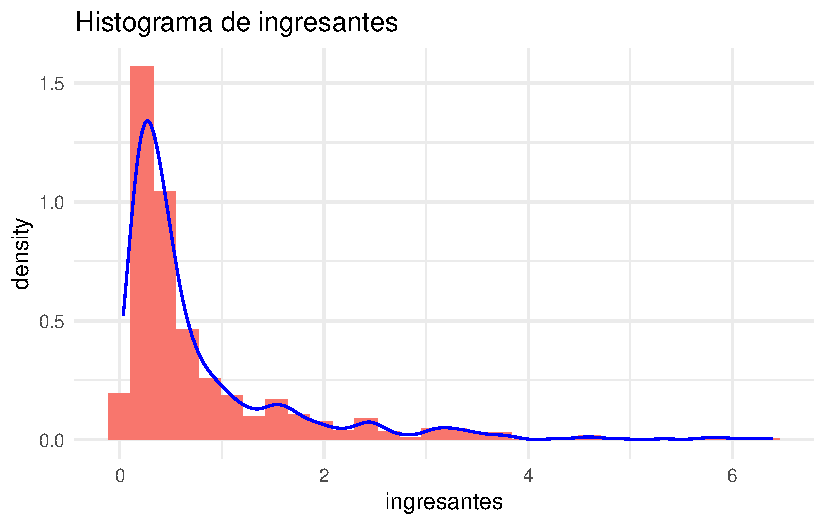
\includegraphics{TP_final_files/figure-pdf/unnamed-chunk-11-1.pdf}

}

\end{figure}

\begin{Shaded}
\begin{Highlighting}[]
\FunctionTok{ggplot}\NormalTok{(df, }\FunctionTok{aes}\NormalTok{(}\AttributeTok{x =}\NormalTok{ ingresantes, }\AttributeTok{y =}\NormalTok{ tasa\_grad, }\AttributeTok{color =}\NormalTok{ privada)) }\SpecialCharTok{+}
  \FunctionTok{geom\_point}\NormalTok{() }\SpecialCharTok{+} 
  \FunctionTok{geom\_smooth}\NormalTok{(}\AttributeTok{formula =} \StringTok{"y \textasciitilde{} x"}\NormalTok{, }\AttributeTok{method =} \StringTok{"lm"}\NormalTok{, }\AttributeTok{se =} \ConstantTok{FALSE}\NormalTok{)}\SpecialCharTok{+}
  \FunctionTok{labs}\NormalTok{(}\AttributeTok{title =} \StringTok{"ingresantes vs Tasa de graduados"}\NormalTok{,}
       \AttributeTok{x =} \StringTok{"ingresantes"}\NormalTok{,}
       \AttributeTok{y =} \StringTok{"\% de graduados"}\NormalTok{)}\SpecialCharTok{+}
  \FunctionTok{theme\_minimal}\NormalTok{()}
\end{Highlighting}
\end{Shaded}

\begin{figure}[H]

{\centering 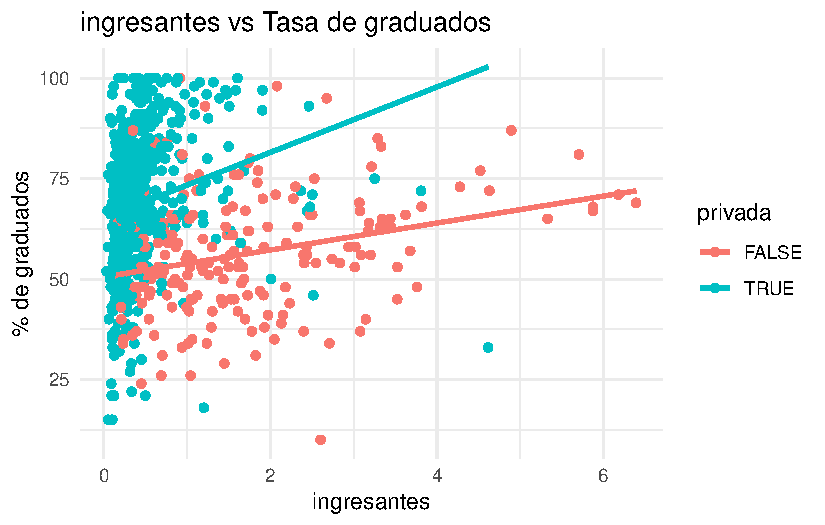
\includegraphics{TP_final_files/figure-pdf/unnamed-chunk-12-1.pdf}

}

\end{figure}

La variable \texttt{ingresante} es de tipo cuantitativa donde hay una
concentración de observaciones grandes para valores bajos de
ingresantes.

No se observa una clara relación lineal contra \texttt{tasa\_grad}

\hypertarget{estudiantes}{%
\subsection{Estudiantes}\label{estudiantes}}

\begin{Shaded}
\begin{Highlighting}[]
\FunctionTok{ggplot}\NormalTok{(df, }\FunctionTok{aes}\NormalTok{(estudiantes))}\SpecialCharTok{+}
  \FunctionTok{geom\_histogram}\NormalTok{(}\AttributeTok{bins =} \DecValTok{30}\NormalTok{, }\FunctionTok{aes}\NormalTok{(}\AttributeTok{fill =} \StringTok{"\#F8766D"}\NormalTok{, }\AttributeTok{y =} \FunctionTok{after\_stat}\NormalTok{(density)))}\SpecialCharTok{+}
  \FunctionTok{geom\_density}\NormalTok{(}\AttributeTok{color =} \StringTok{"blue"}\NormalTok{)}\SpecialCharTok{+}
  \FunctionTok{labs}\NormalTok{(}\AttributeTok{title =} \StringTok{"Histograma de estudiantes"}\NormalTok{,}
       \AttributeTok{x =} \StringTok{"estudiantes"}\NormalTok{)}\SpecialCharTok{+}
  \FunctionTok{theme\_minimal}\NormalTok{()}\SpecialCharTok{+}
  \FunctionTok{theme}\NormalTok{(}\AttributeTok{legend.position =} \StringTok{"none"}\NormalTok{)}
\end{Highlighting}
\end{Shaded}

\begin{figure}[H]

{\centering 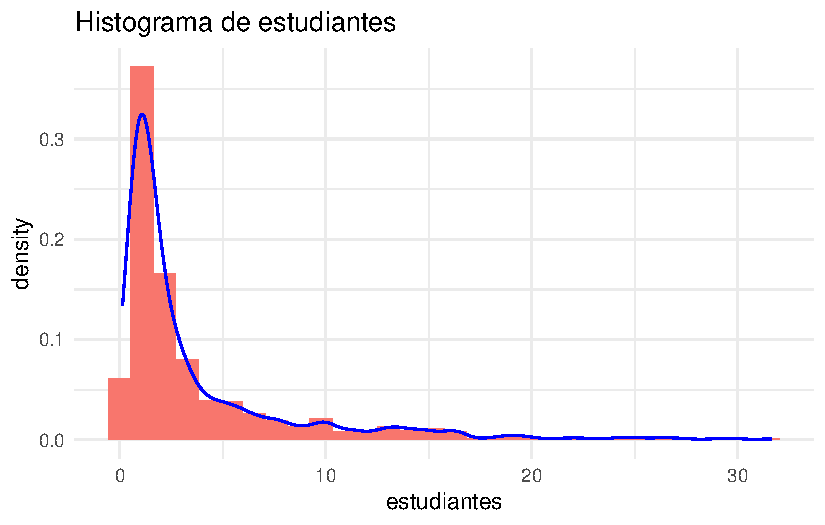
\includegraphics{TP_final_files/figure-pdf/unnamed-chunk-13-1.pdf}

}

\end{figure}

\begin{Shaded}
\begin{Highlighting}[]
\FunctionTok{ggplot}\NormalTok{(df, }\FunctionTok{aes}\NormalTok{(}\AttributeTok{x =}\NormalTok{ estudiantes, }\AttributeTok{y =}\NormalTok{ tasa\_grad, }\AttributeTok{color =}\NormalTok{ privada)) }\SpecialCharTok{+}
  \FunctionTok{geom\_point}\NormalTok{() }\SpecialCharTok{+} 
  \FunctionTok{geom\_smooth}\NormalTok{(}\AttributeTok{formula =} \StringTok{"y \textasciitilde{} x"}\NormalTok{, }\AttributeTok{method =} \StringTok{"lm"}\NormalTok{, }\AttributeTok{se =} \ConstantTok{FALSE}\NormalTok{)}\SpecialCharTok{+}
  \FunctionTok{labs}\NormalTok{(}\AttributeTok{title =} \StringTok{"estudiantes vs Tasa de graduados"}\NormalTok{,}
       \AttributeTok{x =} \StringTok{"estudiantes"}\NormalTok{,}
       \AttributeTok{y =} \StringTok{"\% de graduados"}\NormalTok{)}\SpecialCharTok{+}
  \FunctionTok{theme\_minimal}\NormalTok{()}
\end{Highlighting}
\end{Shaded}

\begin{figure}[H]

{\centering 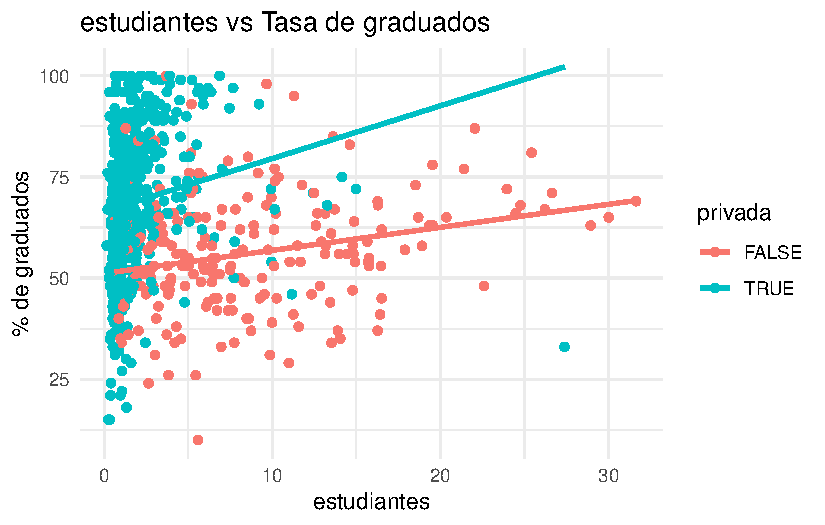
\includegraphics{TP_final_files/figure-pdf/unnamed-chunk-14-1.pdf}

}

\end{figure}

La variable \texttt{estudiantes} es de tipo cuantitativa donde hay una
concentracion de observaciones grandes para valores bajos de
estudiantes.

No se observa una clara relacion lineal contra \texttt{tasa\_grad}

\hypertarget{top-10}{%
\subsection{Top 10}\label{top-10}}

\begin{Shaded}
\begin{Highlighting}[]
\FunctionTok{ggplot}\NormalTok{(df, }\FunctionTok{aes}\NormalTok{(top10))}\SpecialCharTok{+}
  \FunctionTok{geom\_histogram}\NormalTok{(}\AttributeTok{bins =} \DecValTok{30}\NormalTok{, }\FunctionTok{aes}\NormalTok{(}\AttributeTok{fill =} \StringTok{"\#F8766D"}\NormalTok{, }\AttributeTok{y =} \FunctionTok{after\_stat}\NormalTok{(density)))}\SpecialCharTok{+}
  \FunctionTok{geom\_density}\NormalTok{(}\AttributeTok{color =} \StringTok{"blue"}\NormalTok{)}\SpecialCharTok{+}
  \FunctionTok{labs}\NormalTok{(}\AttributeTok{title =} \StringTok{"Histograma de top10"}\NormalTok{,}
       \AttributeTok{x =} \StringTok{"top10"}\NormalTok{)}\SpecialCharTok{+}
  \FunctionTok{theme\_minimal}\NormalTok{()}\SpecialCharTok{+}
  \FunctionTok{theme}\NormalTok{(}\AttributeTok{legend.position =} \StringTok{"none"}\NormalTok{)}
\end{Highlighting}
\end{Shaded}

\begin{figure}[H]

{\centering 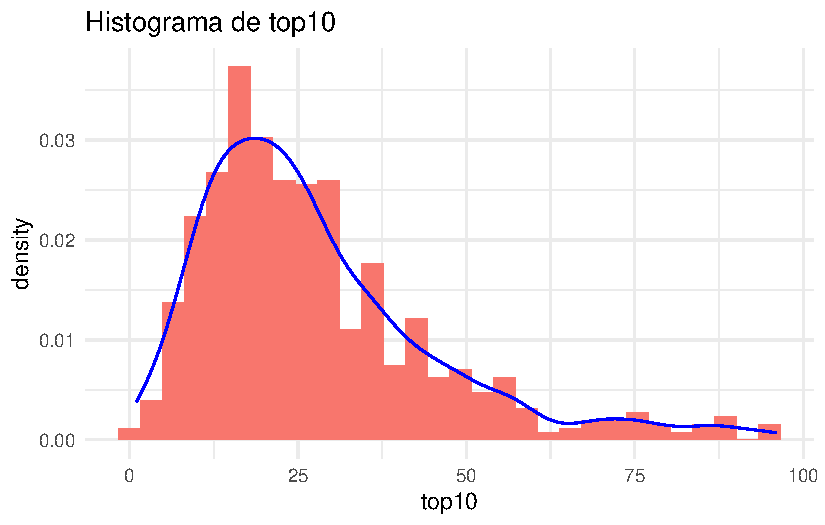
\includegraphics{TP_final_files/figure-pdf/unnamed-chunk-15-1.pdf}

}

\end{figure}

\begin{Shaded}
\begin{Highlighting}[]
\FunctionTok{ggplot}\NormalTok{(df, }\FunctionTok{aes}\NormalTok{(}\AttributeTok{x =}\NormalTok{ top10, }\AttributeTok{y =}\NormalTok{ tasa\_grad, }\AttributeTok{color =}\NormalTok{ privada)) }\SpecialCharTok{+}
  \FunctionTok{geom\_point}\NormalTok{() }\SpecialCharTok{+} 
  \FunctionTok{geom\_smooth}\NormalTok{(}\AttributeTok{formula =} \StringTok{"y \textasciitilde{} x"}\NormalTok{, }\AttributeTok{method =} \StringTok{"lm"}\NormalTok{, }\AttributeTok{se =} \ConstantTok{FALSE}\NormalTok{)}\SpecialCharTok{+}
  \FunctionTok{labs}\NormalTok{(}\AttributeTok{title =} \StringTok{"top10 vs Tasa de graduados"}\NormalTok{,}
       \AttributeTok{x =} \StringTok{"top10"}\NormalTok{,}
       \AttributeTok{y =} \StringTok{"\% de graduados"}\NormalTok{)}\SpecialCharTok{+}
  \FunctionTok{theme\_minimal}\NormalTok{()}
\end{Highlighting}
\end{Shaded}

\begin{figure}[H]

{\centering 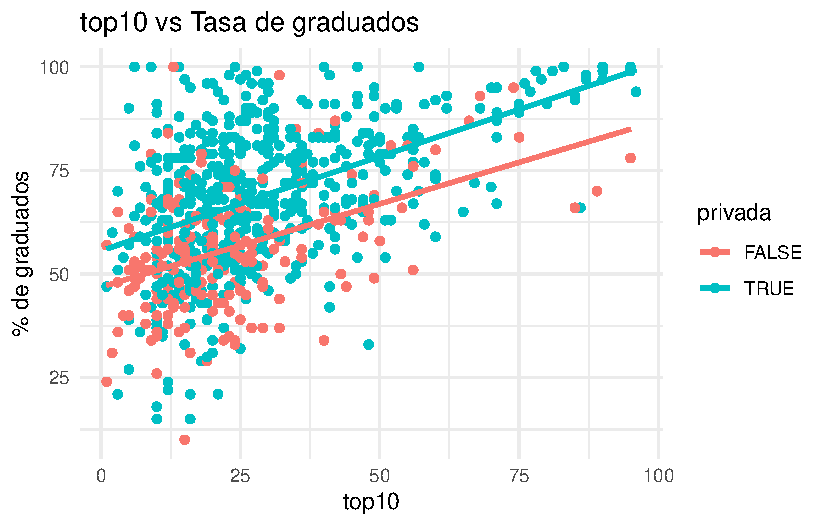
\includegraphics{TP_final_files/figure-pdf/unnamed-chunk-16-1.pdf}

}

\end{figure}

La variable \texttt{top10} es de tipo cuantitativa con las siguientes
metricas estadisticas

\begin{longtable}[]{@{}ll@{}}
\toprule\noalign{}
Variable & Valor \\
\midrule\noalign{}
\endhead
\bottomrule\noalign{}
\endlastfoot
Maximo & \texttt{\{r\}\ round(max(df\$top10),2)} \\
Promedio & \texttt{\{r\}\ round(mean(df\$top10),2)} \\
Minimo & \texttt{\{r\}\ round(min(df\$top10),2)} \\
Desviacion & \texttt{\{r\}\ round(sd(df\$top10),2)} \\
\end{longtable}

Al graficar esta variable con el target notamos una relación lineal
entre ellas pero para valores bajos de porcentaje de top10 hay una mayor
variación entre el valor real con el un valor predicho con una regresión
lineal donde \texttt{tasa\_grad} \textasciitilde{} \texttt{top10}

Otro aspecto de interés es que las regresiones para los dos valores de
la variable \texttt{privada} tienen una pendiente similar, pero
diferente intercepto

\hypertarget{profesores-con-doctorado}{%
\subsection{Profesores con doctorado}\label{profesores-con-doctorado}}

\begin{Shaded}
\begin{Highlighting}[]
\FunctionTok{ggplot}\NormalTok{(df, }\FunctionTok{aes}\NormalTok{(prof\_dr))}\SpecialCharTok{+}
  \FunctionTok{geom\_histogram}\NormalTok{(}\AttributeTok{bins =} \DecValTok{30}\NormalTok{, }\FunctionTok{aes}\NormalTok{(}\AttributeTok{fill =} \StringTok{"\#F8766D"}\NormalTok{, }\AttributeTok{y =} \FunctionTok{after\_stat}\NormalTok{(density)))}\SpecialCharTok{+}
  \FunctionTok{geom\_density}\NormalTok{(}\AttributeTok{color =} \StringTok{"blue"}\NormalTok{)}\SpecialCharTok{+}
  \FunctionTok{labs}\NormalTok{(}\AttributeTok{title =} \StringTok{"Histograma de prof\_dr"}\NormalTok{,}
       \AttributeTok{x =} \StringTok{"prof\_dr"}\NormalTok{)}\SpecialCharTok{+}
  \FunctionTok{theme\_minimal}\NormalTok{()}\SpecialCharTok{+}
  \FunctionTok{theme}\NormalTok{(}\AttributeTok{legend.position =} \StringTok{"none"}\NormalTok{)}
\end{Highlighting}
\end{Shaded}

\begin{figure}[H]

{\centering 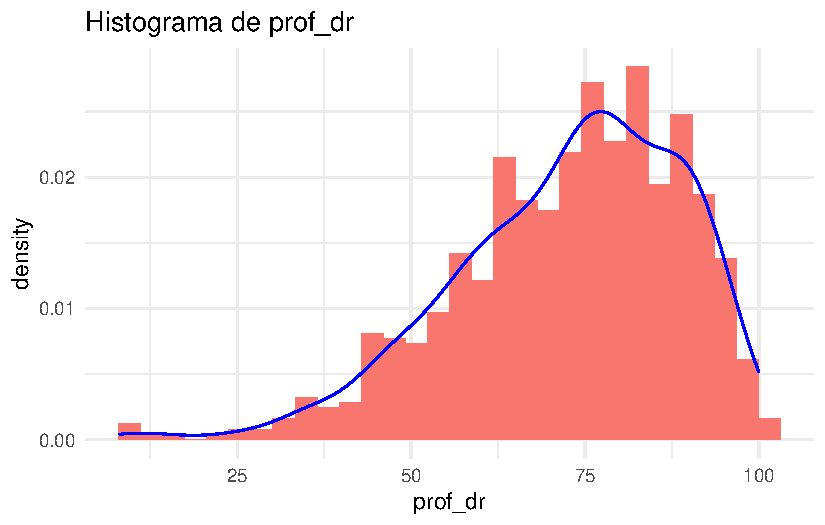
\includegraphics{TP_final_files/figure-pdf/unnamed-chunk-17-1.pdf}

}

\end{figure}

\begin{Shaded}
\begin{Highlighting}[]
\FunctionTok{ggplot}\NormalTok{(df, }\FunctionTok{aes}\NormalTok{(}\AttributeTok{x =}\NormalTok{ prof\_dr, }\AttributeTok{y =}\NormalTok{ tasa\_grad, }\AttributeTok{color =}\NormalTok{ privada)) }\SpecialCharTok{+}
  \FunctionTok{geom\_point}\NormalTok{() }\SpecialCharTok{+} 
  \FunctionTok{geom\_smooth}\NormalTok{(}\AttributeTok{formula =} \StringTok{"y \textasciitilde{} x"}\NormalTok{, }\AttributeTok{method =} \StringTok{"lm"}\NormalTok{, }\AttributeTok{se =} \ConstantTok{FALSE}\NormalTok{)}\SpecialCharTok{+}
  \FunctionTok{labs}\NormalTok{(}\AttributeTok{title =} \StringTok{"prof\_dr vs Tasa de graduados"}\NormalTok{,}
       \AttributeTok{x =} \StringTok{"prof\_dr"}\NormalTok{,}
       \AttributeTok{y =} \StringTok{"\% de graduados"}\NormalTok{)}\SpecialCharTok{+}
  \FunctionTok{theme\_minimal}\NormalTok{()}
\end{Highlighting}
\end{Shaded}

\begin{figure}[H]

{\centering 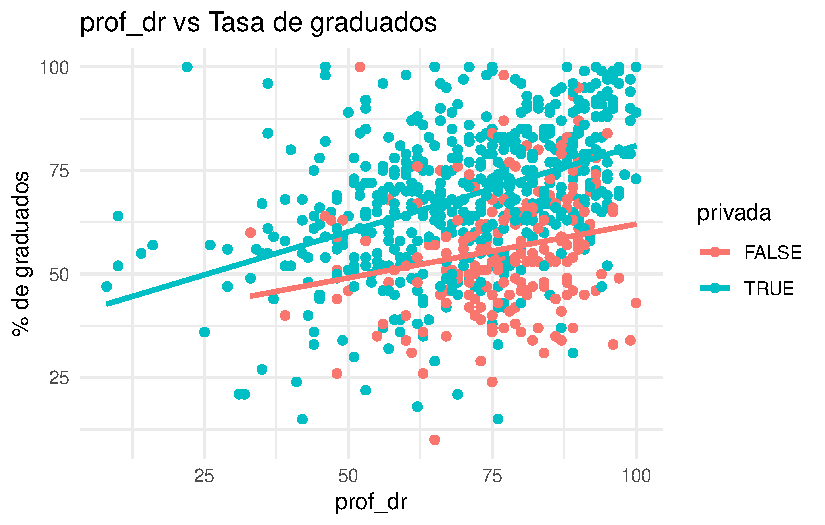
\includegraphics{TP_final_files/figure-pdf/unnamed-chunk-18-1.pdf}

}

\end{figure}

La variable \texttt{prof\_dr} es de tipo cuantitativa con las siguientes
métricas estadísticas

\begin{longtable}[]{@{}ll@{}}
\toprule\noalign{}
Variable & Valor \\
\midrule\noalign{}
\endhead
\bottomrule\noalign{}
\endlastfoot
Maximo & \texttt{\{r\}\ round(max(df\$prof\_dr),2)} \\
Promedio & \texttt{\{r\}\ round(mean(df\$prof\_dr),2)} \\
Minimo & \texttt{\{r\}\ round(min(df\$prof\_dr),2)} \\
Desviacion & \texttt{\{r\}\ round(sd(df\$prof\_dr),2)} \\
\end{longtable}

Al graficar esta variable con el target no se observa una clara relación
lineal. Un aspecto de interés es que las regresiones para los dos
valores de la variable \texttt{privada} tienen una pendiente similar,
pero diferente intercepto

\hypertarget{razon-de-alumnos-por-profesores}{%
\subsection{Razon de alumnos por
profesores}\label{razon-de-alumnos-por-profesores}}

\begin{Shaded}
\begin{Highlighting}[]
\FunctionTok{ggplot}\NormalTok{(df, }\FunctionTok{aes}\NormalTok{(razon))}\SpecialCharTok{+}
  \FunctionTok{geom\_histogram}\NormalTok{(}\AttributeTok{bins =} \DecValTok{30}\NormalTok{, }\FunctionTok{aes}\NormalTok{(}\AttributeTok{fill =} \StringTok{"\#F8766D"}\NormalTok{, }\AttributeTok{y =} \FunctionTok{after\_stat}\NormalTok{(density)))}\SpecialCharTok{+}
  \FunctionTok{geom\_density}\NormalTok{(}\AttributeTok{color =} \StringTok{"blue"}\NormalTok{)}\SpecialCharTok{+}
  \FunctionTok{labs}\NormalTok{(}\AttributeTok{title =} \StringTok{"Histograma de razon"}\NormalTok{,}
       \AttributeTok{x =} \StringTok{"razon"}\NormalTok{)}\SpecialCharTok{+}
  \FunctionTok{theme\_minimal}\NormalTok{()}\SpecialCharTok{+}
  \FunctionTok{theme}\NormalTok{(}\AttributeTok{legend.position =} \StringTok{"none"}\NormalTok{)}
\end{Highlighting}
\end{Shaded}

\begin{figure}[H]

{\centering 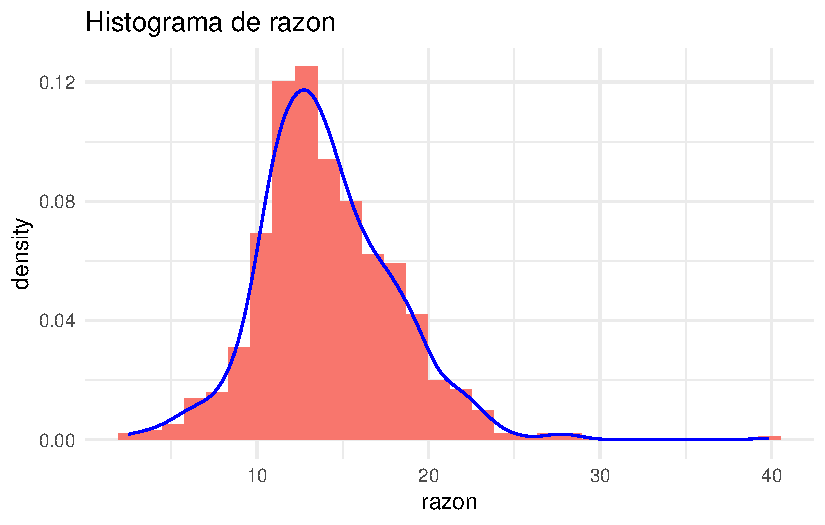
\includegraphics{TP_final_files/figure-pdf/unnamed-chunk-19-1.pdf}

}

\end{figure}

\begin{Shaded}
\begin{Highlighting}[]
\FunctionTok{ggplot}\NormalTok{(df, }\FunctionTok{aes}\NormalTok{(}\AttributeTok{x =}\NormalTok{ razon, }\AttributeTok{y =}\NormalTok{ tasa\_grad, }\AttributeTok{color =}\NormalTok{ privada)) }\SpecialCharTok{+}
  \FunctionTok{geom\_point}\NormalTok{() }\SpecialCharTok{+} 
  \FunctionTok{geom\_smooth}\NormalTok{(}\AttributeTok{formula =} \StringTok{"y \textasciitilde{} x"}\NormalTok{, }\AttributeTok{method =} \StringTok{"lm"}\NormalTok{, }\AttributeTok{se =} \ConstantTok{FALSE}\NormalTok{)}\SpecialCharTok{+}
  \FunctionTok{labs}\NormalTok{(}\AttributeTok{title =} \StringTok{"razon vs Tasa de graduados"}\NormalTok{,}
       \AttributeTok{x =} \StringTok{"razon"}\NormalTok{,}
       \AttributeTok{y =} \StringTok{"\% de graduados"}\NormalTok{)}\SpecialCharTok{+}
  \FunctionTok{theme\_minimal}\NormalTok{()}
\end{Highlighting}
\end{Shaded}

\begin{figure}[H]

{\centering 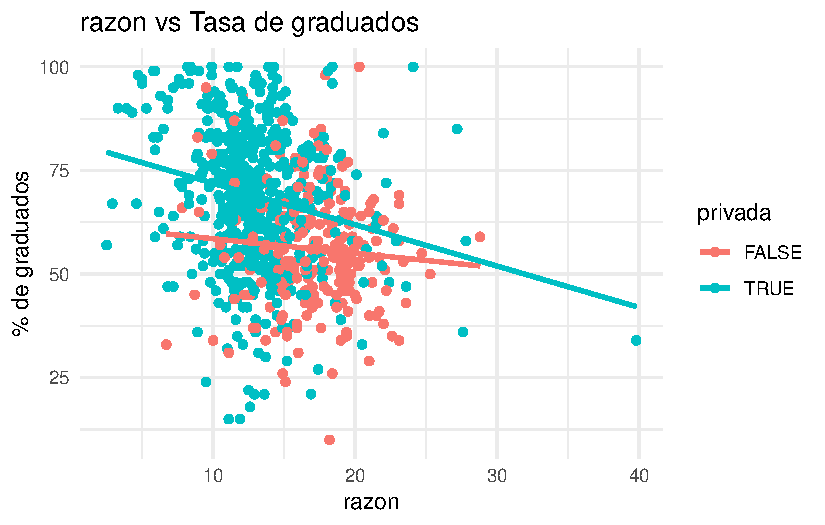
\includegraphics{TP_final_files/figure-pdf/unnamed-chunk-20-1.pdf}

}

\end{figure}

La variable \texttt{razon} es de tipo cuantitativa con las siguientes
métricas estadísticas

\begin{longtable}[]{@{}ll@{}}
\toprule\noalign{}
Variable & Valor \\
\midrule\noalign{}
\endhead
\bottomrule\noalign{}
\endlastfoot
Maximo & \texttt{\{r\}\ round(max(df\$razon),2)} \\
Promedio & \texttt{\{r\}\ round(mean(df\$razon),2)} \\
Minimo & \texttt{\{r\}\ round(min(df\$razon),2)} \\
Desviacion & \texttt{\{r\}\ round(sd(df\$razon),2)} \\
\end{longtable}

La variable estudiantes es de tipo cuantitativa donde hay una
concentración de observaciones grandes para valores entre 10 y 15.

No se observa una clara relación lineal contra tasa\_grad

\hypertarget{tasa-de-graduados}{%
\subsection{Tasa de graduados}\label{tasa-de-graduados}}

\begin{Shaded}
\begin{Highlighting}[]
\FunctionTok{ggplot}\NormalTok{(df, }\FunctionTok{aes}\NormalTok{(tasa\_grad))}\SpecialCharTok{+}
  \FunctionTok{geom\_histogram}\NormalTok{(}\AttributeTok{bins =} \DecValTok{30}\NormalTok{, }\FunctionTok{aes}\NormalTok{(}\AttributeTok{fill =} \StringTok{"\#F8766D"}\NormalTok{, }\AttributeTok{y =} \FunctionTok{after\_stat}\NormalTok{(density)))}\SpecialCharTok{+}
  \FunctionTok{geom\_density}\NormalTok{(}\AttributeTok{color =} \StringTok{"blue"}\NormalTok{)}\SpecialCharTok{+}
  \FunctionTok{labs}\NormalTok{(}\AttributeTok{title =} \StringTok{"Histograma de tasa\_grad"}\NormalTok{,}
       \AttributeTok{x =} \StringTok{"tasa\_grad"}\NormalTok{)}\SpecialCharTok{+}
  \FunctionTok{theme\_minimal}\NormalTok{()}\SpecialCharTok{+}
  \FunctionTok{theme}\NormalTok{(}\AttributeTok{legend.position =} \StringTok{"none"}\NormalTok{)}
\end{Highlighting}
\end{Shaded}

\begin{figure}[H]

{\centering 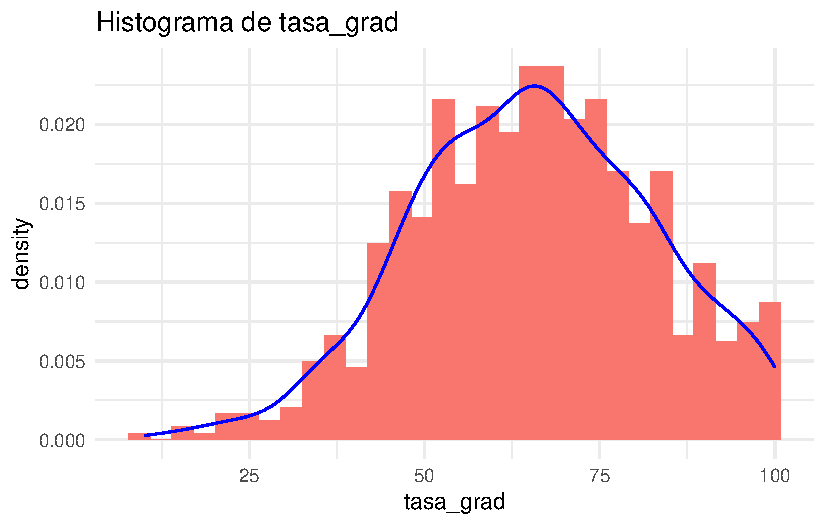
\includegraphics{TP_final_files/figure-pdf/unnamed-chunk-21-1.pdf}

}

\end{figure}

La variable \texttt{tasa\_grad} es de tipo cuantitativa con las
siguientes métricas estadísticas y es la variable target de nuestro
análisis.

\begin{longtable}[]{@{}ll@{}}
\toprule\noalign{}
Variable & Valor \\
\midrule\noalign{}
\endhead
\bottomrule\noalign{}
\endlastfoot
Maximo & \texttt{\{r\}\ round(max(df\$tasa\_grad),2)} \\
Promedio & \texttt{\{r\}\ round(mean(df\$tasa\_grad),2)} \\
Minimo & \texttt{\{r\}\ round(min(df\$tasa\_grad),2)} \\
Desviacion & \texttt{\{r\}\ round(sd(df\$tasa\_grad),2)} \\
\end{longtable}

\hypertarget{regresiuxf3n-lineal}{%
\section{Regresión Lineal}\label{regresiuxf3n-lineal}}

\hypertarget{divisiuxf3n-en-entrenamiento-y-prueba}{%
\subsection{División en entrenamiento y
prueba}\label{divisiuxf3n-en-entrenamiento-y-prueba}}

\begin{Shaded}
\begin{Highlighting}[]
\FunctionTok{set.seed}\NormalTok{(}\DecValTok{1234}\NormalTok{)}
\NormalTok{filas\_train }\OtherTok{\textless{}{-}} \FunctionTok{sample}\NormalTok{(}\AttributeTok{x =} \DecValTok{1}\SpecialCharTok{:}\FunctionTok{nrow}\NormalTok{(df), }\AttributeTok{size =} \FunctionTok{nrow}\NormalTok{(df)}\SpecialCharTok{*}\FloatTok{0.7}\NormalTok{) }\CommentTok{\#asignacion aleatoria}

\NormalTok{df\_train }\OtherTok{\textless{}{-}} \FunctionTok{slice}\NormalTok{(df, filas\_train)}
\NormalTok{df\_test }\OtherTok{\textless{}{-}} \FunctionTok{slice}\NormalTok{(df, }\SpecialCharTok{{-}}\NormalTok{filas\_train)}
\end{Highlighting}
\end{Shaded}

\hypertarget{ajustes-de-modelos}{%
\subsection{Ajustes de modelos}\label{ajustes-de-modelos}}

El \textbf{primer modelo} propuesto surge de aplicar un método de
selección \emph{stepwise} considerando solamente las variables
originales, sin interacciones.

\begin{Shaded}
\begin{Highlighting}[]
\NormalTok{mod1 }\OtherTok{\textless{}{-}} \FunctionTok{stepAIC}\NormalTok{(}
  \AttributeTok{object =} \FunctionTok{lm}\NormalTok{(tasa\_grad }\SpecialCharTok{\textasciitilde{}} \DecValTok{1}\NormalTok{, }\AttributeTok{data =}\NormalTok{ df\_train), }\CommentTok{\#punto de partida}
  \AttributeTok{scope =} \FunctionTok{list}\NormalTok{(}\AttributeTok{upper =} \FunctionTok{lm}\NormalTok{(tasa\_grad }\SpecialCharTok{\textasciitilde{}}\NormalTok{ ., }\AttributeTok{data =}\NormalTok{ df\_train)), }\CommentTok{\#máximo modelo posible}
  \AttributeTok{direction =} \StringTok{"both"}\NormalTok{, }\CommentTok{\#método de selección}
  \AttributeTok{trace =} \ConstantTok{FALSE}\NormalTok{, }\CommentTok{\#para no imprimir resultados parciales}
  \AttributeTok{k =} \DecValTok{2}\NormalTok{, }\CommentTok{\#penalización a emplear (2 = AIC, log(n) = BIC)}
  \AttributeTok{steps =} \DecValTok{1000} \CommentTok{\#máximo nro de pasos}
\NormalTok{)}
\NormalTok{mod1}
\end{Highlighting}
\end{Shaded}

\begin{verbatim}

Call:
lm(formula = tasa_grad ~ cuota + top10, data = df_train)

Coefficients:
(Intercept)        cuota        top10  
    39.1618       1.8600       0.2487  
\end{verbatim}

El \textbf{segundo modelo} también surge de aplicar el método
\emph{stepwise} pero considerando como modelo maximal aquel con todas
las interacciones de segundo orden.

\begin{Shaded}
\begin{Highlighting}[]
\NormalTok{mod2 }\OtherTok{\textless{}{-}} \FunctionTok{stepAIC}\NormalTok{(}
  \AttributeTok{object =} \FunctionTok{lm}\NormalTok{(tasa\_grad }\SpecialCharTok{\textasciitilde{}} \DecValTok{1}\NormalTok{, }\AttributeTok{data =}\NormalTok{ df\_train), }\CommentTok{\#punto de partida}
  \AttributeTok{scope =} \FunctionTok{list}\NormalTok{(}\AttributeTok{upper =} \FunctionTok{lm}\NormalTok{(tasa\_grad }\SpecialCharTok{\textasciitilde{}}\NormalTok{ .}\SpecialCharTok{\^{}}\DecValTok{2}\NormalTok{, }\AttributeTok{data =}\NormalTok{ df\_train)), }\CommentTok{\#máximo modelo posible}
  \AttributeTok{direction =} \StringTok{"both"}\NormalTok{, }\CommentTok{\#método de selección}
  \AttributeTok{trace =} \ConstantTok{FALSE}\NormalTok{, }\CommentTok{\#para no imprimir resultados parciales}
  \AttributeTok{k =} \DecValTok{2}\NormalTok{, }\CommentTok{\#penalización a emplear (2 = AIC, log(n) = BIC)}
  \AttributeTok{steps =} \DecValTok{1000} \CommentTok{\#máximo nro de pasos}
\NormalTok{)}
\NormalTok{mod2}
\end{Highlighting}
\end{Shaded}

\begin{verbatim}

Call:
lm(formula = tasa_grad ~ cuota + top10 + cuota:top10, data = df_train)

Coefficients:
(Intercept)        cuota        top10  cuota:top10  
   33.99731      2.33018      0.43030     -0.01453  
\end{verbatim}

El \textbf{tercer modelo} surge de aplicar la técnica de mejores
subconjuntos. Visto que el modelo anterior incluye tres términos (dos
efectos principales y una interacción entre ellos) se elige el mejor
modelo con 3 variables explicativas.

\begin{Shaded}
\begin{Highlighting}[]
\NormalTok{mejorsub }\OtherTok{\textless{}{-}} \FunctionTok{regsubsets}\NormalTok{(}\AttributeTok{x =}\NormalTok{ tasa\_grad }\SpecialCharTok{\textasciitilde{}}\NormalTok{ ., }\AttributeTok{data =}\NormalTok{ df\_train)}
\FunctionTok{summary}\NormalTok{(mejorsub)}
\end{Highlighting}
\end{Shaded}

\begin{verbatim}
Subset selection object
Call: regsubsets.formula(x = tasa_grad ~ ., data = df_train)
8 Variables  (and intercept)
             Forced in Forced out
privadaTRUE      FALSE      FALSE
aplicaciones     FALSE      FALSE
ingresantes      FALSE      FALSE
estudiantes      FALSE      FALSE
top10            FALSE      FALSE
cuota            FALSE      FALSE
prof_dr          FALSE      FALSE
razon            FALSE      FALSE
1 subsets of each size up to 8
Selection Algorithm: exhaustive
         privadaTRUE aplicaciones ingresantes estudiantes top10 cuota prof_dr
1  ( 1 ) " "         " "          " "         " "         " "   "*"   " "    
2  ( 1 ) " "         " "          " "         " "         "*"   "*"   " "    
3  ( 1 ) "*"         " "          " "         " "         "*"   "*"   " "    
4  ( 1 ) " "         "*"          " "         "*"         "*"   "*"   " "    
5  ( 1 ) "*"         "*"          " "         "*"         "*"   "*"   " "    
6  ( 1 ) "*"         "*"          " "         "*"         "*"   "*"   "*"    
7  ( 1 ) "*"         "*"          "*"         "*"         "*"   "*"   "*"    
8  ( 1 ) "*"         "*"          "*"         "*"         "*"   "*"   "*"    
         razon
1  ( 1 ) " "  
2  ( 1 ) " "  
3  ( 1 ) " "  
4  ( 1 ) " "  
5  ( 1 ) " "  
6  ( 1 ) " "  
7  ( 1 ) " "  
8  ( 1 ) "*"  
\end{verbatim}

\begin{Shaded}
\begin{Highlighting}[]
\NormalTok{mod3 }\OtherTok{\textless{}{-}} \FunctionTok{lm}\NormalTok{(tasa\_grad }\SpecialCharTok{\textasciitilde{}}\NormalTok{ privada }\SpecialCharTok{+}\NormalTok{ cuota }\SpecialCharTok{+}\NormalTok{ top10, }\AttributeTok{data =}\NormalTok{ df\_train)}
\end{Highlighting}
\end{Shaded}

\hypertarget{comparaciuxf3n-de-modelos}{%
\subsection{Comparación de modelos}\label{comparaciuxf3n-de-modelos}}

\begin{Shaded}
\begin{Highlighting}[]
\NormalTok{CME }\OtherTok{\textless{}{-}} \ControlFlowTok{function}\NormalTok{(mod) \{ }
\NormalTok{  SSE }\OtherTok{\textless{}{-}} \FunctionTok{sum}\NormalTok{(mod}\SpecialCharTok{$}\NormalTok{residuals}\SpecialCharTok{\^{}}\DecValTok{2}\NormalTok{)}
\NormalTok{  n }\OtherTok{\textless{}{-}} \FunctionTok{length}\NormalTok{(mod}\SpecialCharTok{$}\NormalTok{fitted.values)}
\NormalTok{  SSE }\SpecialCharTok{/}\NormalTok{ (n }\SpecialCharTok{{-}} \DecValTok{1}\NormalTok{) }
\NormalTok{\}}
\NormalTok{PRESS }\OtherTok{\textless{}{-}} \ControlFlowTok{function}\NormalTok{(mod) \{}
  \FunctionTok{sum}\NormalTok{( ( mod}\SpecialCharTok{$}\NormalTok{residuals }\SpecialCharTok{/}\NormalTok{ (}\DecValTok{1} \SpecialCharTok{{-}} \FunctionTok{hatvalues}\NormalTok{(mod)) )}\SpecialCharTok{\^{}}\DecValTok{2}\NormalTok{ )}
\NormalTok{\}}
\NormalTok{Cp }\OtherTok{\textless{}{-}} \ControlFlowTok{function}\NormalTok{(mod) \{ }
\NormalTok{  SSE }\OtherTok{\textless{}{-}} \FunctionTok{sum}\NormalTok{(mod}\SpecialCharTok{$}\NormalTok{residuals}\SpecialCharTok{\^{}}\DecValTok{2}\NormalTok{)}
\NormalTok{  mod\_max }\OtherTok{\textless{}{-}} \FunctionTok{lm}\NormalTok{(tasa\_grad }\SpecialCharTok{\textasciitilde{}}\NormalTok{ .}\SpecialCharTok{\^{}}\DecValTok{2}\NormalTok{, }\AttributeTok{data =}\NormalTok{ df\_train)}
\NormalTok{  SSE\_max }\OtherTok{\textless{}{-}} \FunctionTok{sum}\NormalTok{(mod\_max}\SpecialCharTok{$}\NormalTok{residuals}\SpecialCharTok{\^{}}\DecValTok{2}\NormalTok{) }
\NormalTok{  n }\OtherTok{\textless{}{-}} \FunctionTok{length}\NormalTok{(mod}\SpecialCharTok{$}\NormalTok{fitted.values)}
\NormalTok{  p }\OtherTok{\textless{}{-}} \FunctionTok{length}\NormalTok{(mod}\SpecialCharTok{$}\NormalTok{coefficients)}
\NormalTok{  SSE }\SpecialCharTok{/}\NormalTok{ (SSE\_max }\SpecialCharTok{/}\NormalTok{ (n }\SpecialCharTok{{-}} \DecValTok{1}\NormalTok{)) }\SpecialCharTok{+} \DecValTok{2}\SpecialCharTok{*}\NormalTok{p }\SpecialCharTok{{-}}\NormalTok{ n}
\NormalTok{\}}

\NormalTok{metricas }\OtherTok{\textless{}{-}} \FunctionTok{data.frame}\NormalTok{(}
  \AttributeTok{CME   =} \FunctionTok{c}\NormalTok{( }\FunctionTok{CME}\NormalTok{(mod1),   }\FunctionTok{CME}\NormalTok{(mod2),   }\FunctionTok{CME}\NormalTok{(mod3) ),}
  \AttributeTok{PRESS =} \FunctionTok{c}\NormalTok{( }\FunctionTok{PRESS}\NormalTok{(mod1), }\FunctionTok{PRESS}\NormalTok{(mod2), }\FunctionTok{PRESS}\NormalTok{(mod3) ),}
  \AttributeTok{Cp    =} \FunctionTok{c}\NormalTok{( }\FunctionTok{Cp}\NormalTok{(mod1),    }\FunctionTok{Cp}\NormalTok{(mod2),    }\FunctionTok{Cp}\NormalTok{(mod3) ),}
  \AttributeTok{AIC   =} \FunctionTok{c}\NormalTok{( }\FunctionTok{AIC}\NormalTok{(mod1),   }\FunctionTok{AIC}\NormalTok{(mod2),   }\FunctionTok{AIC}\NormalTok{(mod3) ),}
  \AttributeTok{BIC   =} \FunctionTok{c}\NormalTok{( }\FunctionTok{BIC}\NormalTok{(mod1),   }\FunctionTok{BIC}\NormalTok{(mod2),   }\FunctionTok{BIC}\NormalTok{(mod3) )}
\NormalTok{)}
\NormalTok{metricas}
\end{Highlighting}
\end{Shaded}

\begin{verbatim}
       CME    PRESS       Cp      AIC      BIC
1 177.1570 96972.46 92.92821 4359.097 4376.286
2 175.8549 96567.48 90.29824 4357.091 4378.577
3 176.6482 97082.87 93.11895 4359.535 4381.021
\end{verbatim}

Puede verse que para casi todas las métricas, el mejor modelo (en
términos de desempeño) es el segundo: aquel que considera dos
explicativas y su interacción. Por lo tanto, el modelo seleccionado
queda de la forma:

\[
\texttt{tasa_grad} = \beta_0 + \beta_1 \;\texttt{cuota} + \beta_2 \;\texttt{top10} + \beta_3 \;\texttt{cuota*top10} + \epsilon
\]

\hypertarget{anuxe1lisis-de-residuos}{%
\subsection{Análisis de residuos}\label{anuxe1lisis-de-residuos}}

\begin{Shaded}
\begin{Highlighting}[]
\NormalTok{sel\_mod }\OtherTok{=}\NormalTok{ mod2}

\NormalTok{diagnostico }\OtherTok{=}\NormalTok{ broom}\SpecialCharTok{::}\FunctionTok{augment}\NormalTok{(sel\_mod)}
\end{Highlighting}
\end{Shaded}

\hypertarget{residuos-versus-valores-ajustados}{%
\subsubsection{Residuos versus valores
ajustados}\label{residuos-versus-valores-ajustados}}

\begin{Shaded}
\begin{Highlighting}[]
\FunctionTok{ggplot}\NormalTok{(}\AttributeTok{data =}\NormalTok{ diagnostico) }\SpecialCharTok{+} 
    \FunctionTok{aes}\NormalTok{(}\AttributeTok{x =}\NormalTok{ .fitted, }\AttributeTok{y =}\NormalTok{ .resid) }\SpecialCharTok{+} 
    \FunctionTok{geom\_point}\NormalTok{(}\AttributeTok{alpha =} \FloatTok{0.6}\NormalTok{) }\SpecialCharTok{+}
    \FunctionTok{geom\_hline}\NormalTok{(}\FunctionTok{aes}\NormalTok{(}\AttributeTok{yintercept =} \DecValTok{0}\NormalTok{, }\AttributeTok{color =} \StringTok{"red"}\NormalTok{)) }\SpecialCharTok{+}
    \FunctionTok{xlab}\NormalTok{(}\StringTok{"Valores Ajustados"}\NormalTok{) }\SpecialCharTok{+}
    \FunctionTok{ylab}\NormalTok{(}\StringTok{"Residuos"}\NormalTok{) }\SpecialCharTok{+}
    \FunctionTok{theme\_bw}\NormalTok{()}\SpecialCharTok{+}
    \FunctionTok{theme}\NormalTok{(}\AttributeTok{legend.position =} \StringTok{"none"}\NormalTok{,}
      \AttributeTok{axis.title =} \FunctionTok{element\_text}\NormalTok{(}\AttributeTok{face =} \StringTok{"bold"}\NormalTok{))}
\end{Highlighting}
\end{Shaded}

\begin{figure}[H]

{\centering 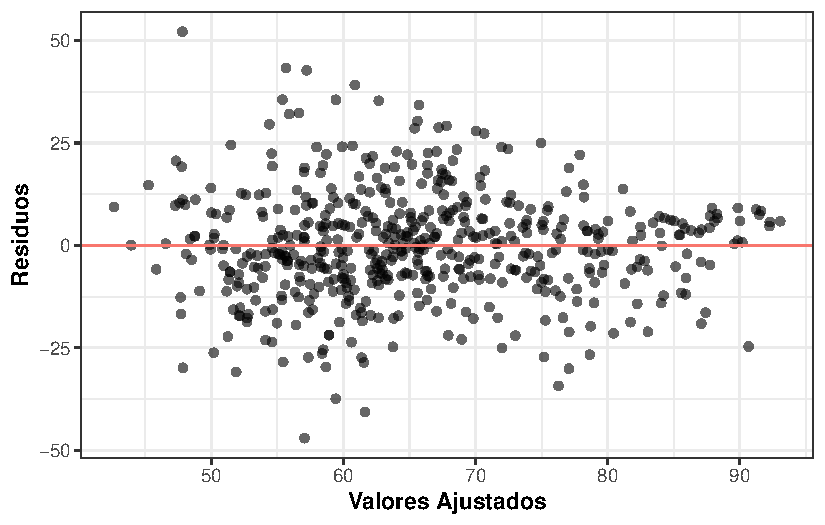
\includegraphics{TP_final_files/figure-pdf/unnamed-chunk-29-1.pdf}

}

\end{figure}

Se puede ver que la variancia de los residuos no es constante para todos
los valores ajustados. En particular, se evidencia una mayor
variabilidad para tasas de graduación predichas en el rango 55\% a 65\%.

La hipótesis anterior puede evaluarse mediante el test de Breusch-Pagan.

\begin{Shaded}
\begin{Highlighting}[]
\NormalTok{lmtest}\SpecialCharTok{::}\FunctionTok{bptest}\NormalTok{(sel\_mod)}
\end{Highlighting}
\end{Shaded}

\begin{verbatim}

    studentized Breusch-Pagan test

data:  sel_mod
BP = 11.965, df = 3, p-value = 0.007503
\end{verbatim}

Como el p-value resulta inferior al nivel de significación 5\%, se
rechaza la hipótesis nula, indicando que posiblemente no se esté
cumpliendo el supuesto de homocedasticidad de los residuos.

\hypertarget{residuos-estandarizados}{%
\subsubsection{Residuos estandarizados}\label{residuos-estandarizados}}

\begin{Shaded}
\begin{Highlighting}[]
\NormalTok{diagnostico}\SpecialCharTok{$}\NormalTok{id }\OtherTok{\textless{}{-}} \FunctionTok{seq}\NormalTok{(}\DecValTok{1}\SpecialCharTok{:}\FunctionTok{nrow}\NormalTok{(diagnostico))}

\FunctionTok{ggplot}\NormalTok{(}\AttributeTok{data =}\NormalTok{ diagnostico) }\SpecialCharTok{+}
  \FunctionTok{aes}\NormalTok{(}\AttributeTok{x =}\NormalTok{ id, }\AttributeTok{y =}\NormalTok{ .std.resid) }\SpecialCharTok{+} 
  \FunctionTok{geom\_point}\NormalTok{(}\AttributeTok{alpha =} \FloatTok{0.6}\NormalTok{) }\SpecialCharTok{+}
  \FunctionTok{geom\_hline}\NormalTok{(}\FunctionTok{aes}\NormalTok{(}\AttributeTok{yintercept =} \DecValTok{0}\NormalTok{, }\AttributeTok{color =} \StringTok{"red"}\NormalTok{)) }\SpecialCharTok{+}
  \FunctionTok{geom\_hline}\NormalTok{(}\FunctionTok{aes}\NormalTok{(}\AttributeTok{yintercept =} \SpecialCharTok{{-}}\DecValTok{3}\NormalTok{, }\AttributeTok{color =} \StringTok{"red"}\NormalTok{)) }\SpecialCharTok{+}
  \FunctionTok{geom\_hline}\NormalTok{(}\FunctionTok{aes}\NormalTok{(}\AttributeTok{yintercept =} \DecValTok{3}\NormalTok{, }\AttributeTok{color =} \StringTok{"red"}\NormalTok{)) }\SpecialCharTok{+}
  \FunctionTok{xlab}\NormalTok{(}\StringTok{"Observación"}\NormalTok{) }\SpecialCharTok{+}
  \FunctionTok{ylab}\NormalTok{(}\StringTok{"Residuos estandarizados"}\NormalTok{) }\SpecialCharTok{+}
  \FunctionTok{theme\_bw}\NormalTok{() }\SpecialCharTok{+}
  \FunctionTok{theme}\NormalTok{(}\AttributeTok{legend.position =} \StringTok{"none"}\NormalTok{,}
        \AttributeTok{axis.title =} \FunctionTok{element\_text}\NormalTok{(}\AttributeTok{face =} \StringTok{"bold"}\NormalTok{))}
\end{Highlighting}
\end{Shaded}

\begin{figure}[H]

{\centering 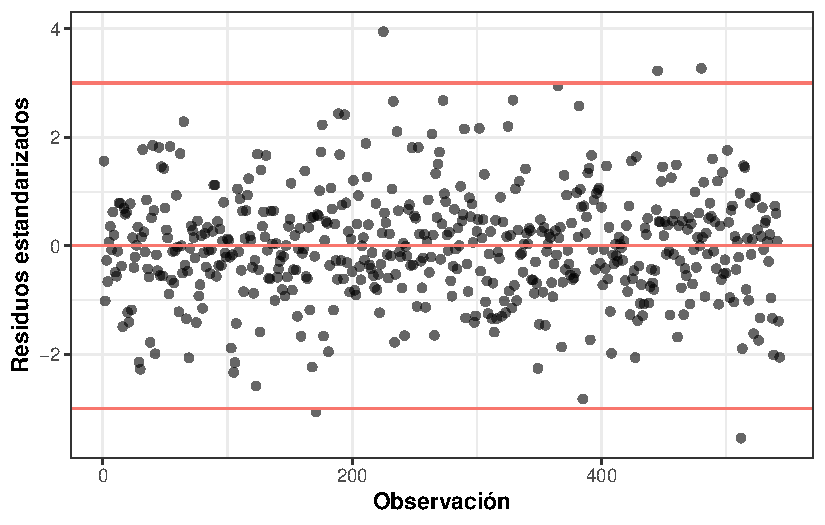
\includegraphics{TP_final_files/figure-pdf/unnamed-chunk-31-1.pdf}

}

\end{figure}

Se encuentran 5 valores con residuos estandarizados mayores a 3
unidades, en valor absoluto. Esto corresponde a un 0.92\% de la
totalidad de las observaciones de entrenamiento.

\hypertarget{residuos-press}{%
\subsubsection{Residuos PRESS}\label{residuos-press}}

\begin{Shaded}
\begin{Highlighting}[]
\NormalTok{diagnostico}\SpecialCharTok{$}\NormalTok{press }\OtherTok{\textless{}{-}}\NormalTok{ qpcR}\SpecialCharTok{::}\FunctionTok{PRESS}\NormalTok{(sel\_mod, }\AttributeTok{verbose=}\ConstantTok{FALSE}\NormalTok{)}\SpecialCharTok{$}\NormalTok{residuals}

\FunctionTok{ggplot}\NormalTok{(}\AttributeTok{data =}\NormalTok{ diagnostico) }\SpecialCharTok{+} 
  \FunctionTok{aes}\NormalTok{(}\AttributeTok{x =}\NormalTok{ id, }\AttributeTok{y =}\NormalTok{ press) }\SpecialCharTok{+} 
  \FunctionTok{geom\_bar}\NormalTok{(}\AttributeTok{stat=}\StringTok{"identity"}\NormalTok{)}\SpecialCharTok{+}
  \FunctionTok{geom\_hline}\NormalTok{(}\FunctionTok{aes}\NormalTok{(}\AttributeTok{yintercept =} \DecValTok{0}\NormalTok{, }\AttributeTok{color =} \StringTok{"red"}\NormalTok{)) }\SpecialCharTok{+}
  \FunctionTok{xlab}\NormalTok{(}\StringTok{"Observación"}\NormalTok{) }\SpecialCharTok{+}
  \FunctionTok{ylab}\NormalTok{(}\StringTok{"PRESS"}\NormalTok{) }\SpecialCharTok{+}
  \FunctionTok{theme\_bw}\NormalTok{() }\SpecialCharTok{+}
  \FunctionTok{theme}\NormalTok{(}\AttributeTok{legend.position =} \StringTok{"none"}\NormalTok{,}
        \AttributeTok{axis.title =} \FunctionTok{element\_text}\NormalTok{(}\AttributeTok{face =} \StringTok{"bold"}\NormalTok{))}
\end{Highlighting}
\end{Shaded}

\begin{figure}[H]

{\centering 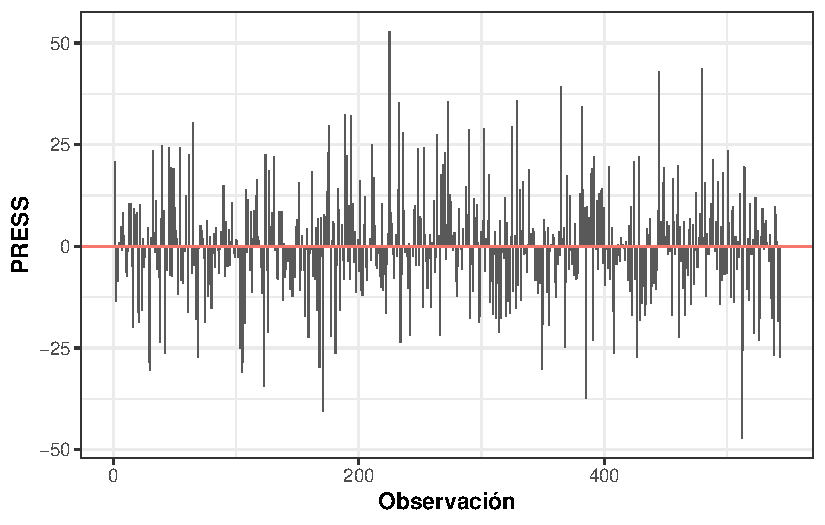
\includegraphics{TP_final_files/figure-pdf/unnamed-chunk-32-1.pdf}

}

\end{figure}

No se ve ninguna observación que arroje un residuo PRESS
considerablemente mayor (en valor absoluto) al resto.

\hypertarget{anuxe1lisis-de-normalidad}{%
\subsubsection{Análisis de normalidad}\label{anuxe1lisis-de-normalidad}}

\begin{Shaded}
\begin{Highlighting}[]
\FunctionTok{plot}\NormalTok{(sel\_mod,}\DecValTok{2}\NormalTok{)}
\end{Highlighting}
\end{Shaded}

\begin{figure}[H]

{\centering 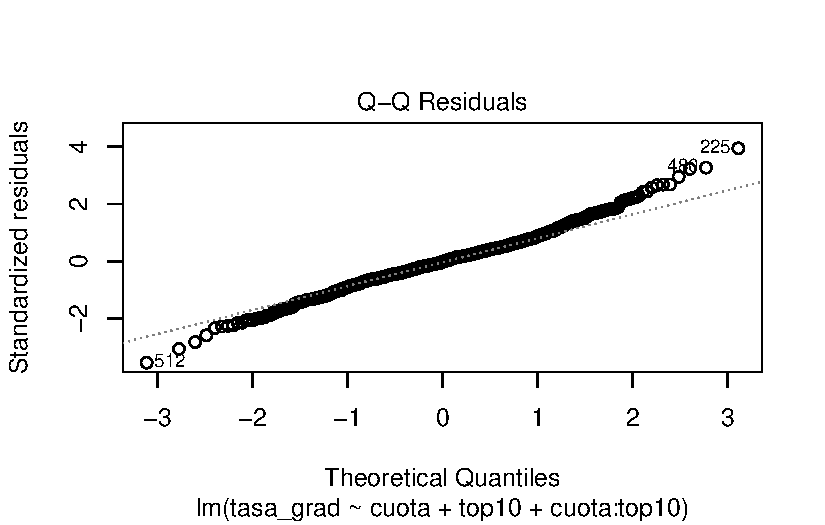
\includegraphics{TP_final_files/figure-pdf/unnamed-chunk-33-1.pdf}

}

\end{figure}

\begin{Shaded}
\begin{Highlighting}[]
\NormalTok{nortest}\SpecialCharTok{::}\FunctionTok{ad.test}\NormalTok{(sel\_mod}\SpecialCharTok{$}\NormalTok{residuals)}
\end{Highlighting}
\end{Shaded}

\begin{verbatim}

    Anderson-Darling normality test

data:  sel_mod$residuals
A = 1.6877, p-value = 0.0002482
\end{verbatim}

Dado que el p-value es inferior al nivel de significación del 5\%, se
rechaza la hipótesis nula de distribución Normal para los errores.

\hypertarget{anuxe1lisis-de-colinealidad}{%
\subsubsection{Análisis de
colinealidad}\label{anuxe1lisis-de-colinealidad}}

\begin{Shaded}
\begin{Highlighting}[]
\NormalTok{car}\SpecialCharTok{::}\FunctionTok{vif}\NormalTok{(sel\_mod)}
\end{Highlighting}
\end{Shaded}

\begin{verbatim}
there are higher-order terms (interactions) in this model
consider setting type = 'predictor'; see ?vif
\end{verbatim}

\begin{verbatim}
      cuota       top10 cuota:top10 
   4.178070    9.384239   16.856884 
\end{verbatim}

Los términos \texttt{top10} y \texttt{cuota:top10} presentan un valor de
VIF mayor a 5 unidades. Esto indicaría una colinealidad entre estos
términos, lo cual resulta lógico dado que el segundo término refiere a
la interacción entre el primer término y la variable explicativa
restante. De hecho, puede verse que los valores de VIF para el modelo
sin interacción se ven reducidos.

\begin{Shaded}
\begin{Highlighting}[]
\NormalTok{car}\SpecialCharTok{::}\FunctionTok{vif}\NormalTok{(mod1)}
\end{Highlighting}
\end{Shaded}

\begin{verbatim}
  cuota   top10 
1.46823 1.46823 
\end{verbatim}

\hypertarget{interpretaciuxf3n-de-los-predictores}{%
\subsection{Interpretación de los
predictores}\label{interpretaciuxf3n-de-los-predictores}}

\begin{Shaded}
\begin{Highlighting}[]
\FunctionTok{summary}\NormalTok{(sel\_mod)}
\end{Highlighting}
\end{Shaded}

\begin{verbatim}

Call:
lm(formula = tasa_grad ~ cuota + top10 + cuota:top10, data = df_train)

Residuals:
    Min      1Q  Median      3Q     Max 
-47.054  -7.871  -0.285   7.113  52.186 

Coefficients:
             Estimate Std. Error t value Pr(>|t|)    
(Intercept) 33.997311   3.043330  11.171  < 2e-16 ***
cuota        2.330176   0.292218   7.974 9.24e-15 ***
top10        0.430303   0.098965   4.348 1.64e-05 ***
cuota:top10 -0.014531   0.007274  -1.998   0.0462 *  
---
Signif. codes:  0 '***' 0.001 '**' 0.01 '*' 0.05 '.' 0.1 ' ' 1

Residual standard error: 13.3 on 539 degrees of freedom
Multiple R-squared:  0.3907,    Adjusted R-squared:  0.3873 
F-statistic: 115.2 on 3 and 539 DF,  p-value: < 2.2e-16
\end{verbatim}

Los tres términos reusltan significativos al 5\%. Por lo tanto, debido a
la presencia de interacción, las interpretaciones de los coeficientes
del modelo son las siguientes:

\begin{itemize}
\item
  Aumentar mil dólares la cuota se asocia con un incremento promedio en
  la tasa de graduación igual a \texttt{2,33\ -\ 0,015\ *\ top10}
  unidades porcentuales.
\item
  Aumentar en una unidad porcentual el porcentaje de ingresantes que
  fueron parte del top 10\% de estudiantes en sus escuelas secundarias
  se asocia con un incremento promedio en la tasa de graduación igual a
  \texttt{0,43\ -\ 0,015\ *\ top10} unidades porcentuales.
\end{itemize}

\hypertarget{regularizaciuxf3n-y-predicciuxf3n}{%
\section{Regularización y
Predicción}\label{regularizaciuxf3n-y-predicciuxf3n}}

\hypertarget{ajuste-con-tuxe9cnica-ridge}{%
\subsection{Ajuste con técnica
Ridge}\label{ajuste-con-tuxe9cnica-ridge}}

\begin{Shaded}
\begin{Highlighting}[]
\FunctionTok{set.seed}\NormalTok{(}\DecValTok{12343}\NormalTok{)}

\NormalTok{X\_train }\OtherTok{=} \FunctionTok{model.matrix}\NormalTok{(sel\_mod)[,}\SpecialCharTok{{-}}\DecValTok{1}\NormalTok{]}
  
\NormalTok{Y\_train }\OtherTok{=}\NormalTok{ df\_train}\SpecialCharTok{$}\NormalTok{tasa\_grad}

\NormalTok{mod\_ridge }\OtherTok{=} \FunctionTok{train}\NormalTok{(}
  \AttributeTok{x =}\NormalTok{ X\_train, }\AttributeTok{y=}\NormalTok{ Y\_train,}
  \AttributeTok{method =} \StringTok{"glmnet"}\NormalTok{,}
  \AttributeTok{tuneGrid =} \FunctionTok{expand.grid}\NormalTok{(}\AttributeTok{alpha =} \DecValTok{0}\NormalTok{, }\AttributeTok{lambda =} \FunctionTok{seq}\NormalTok{(}\DecValTok{0}\NormalTok{,}\DecValTok{1}\NormalTok{,}\AttributeTok{by =} \FloatTok{0.1}\NormalTok{)),}
  \AttributeTok{metric =} \StringTok{"RMSE"}\NormalTok{,}
  \AttributeTok{trControl =} \FunctionTok{trainControl}\NormalTok{(}\AttributeTok{method =} \StringTok{"repeatedcv"}\NormalTok{, }\AttributeTok{number =} \DecValTok{5}\NormalTok{, }\AttributeTok{repeats =} \DecValTok{5}\NormalTok{)}
\NormalTok{)}

\NormalTok{lambda\_ridge }\OtherTok{=}\NormalTok{ mod\_ridge}\SpecialCharTok{$}\NormalTok{bestTune[[}\DecValTok{2}\NormalTok{]]}

\NormalTok{mod\_ridge\_sel }\OtherTok{=} \FunctionTok{glmnet}\NormalTok{(}\AttributeTok{x =}\NormalTok{ X\_train, }\AttributeTok{y =}\NormalTok{ Y\_train, }\AttributeTok{alpha =} \DecValTok{0}\NormalTok{, }\AttributeTok{lambda =}\NormalTok{ lambda\_ridge)}

\NormalTok{lambda\_ridge}
\end{Highlighting}
\end{Shaded}

\begin{verbatim}
[1] 0.9
\end{verbatim}

\hypertarget{ajuste-con-tuxe9cnica-lasso}{%
\subsection{Ajuste con técnica
Lasso}\label{ajuste-con-tuxe9cnica-lasso}}

\begin{Shaded}
\begin{Highlighting}[]
\FunctionTok{set.seed}\NormalTok{(}\DecValTok{567}\NormalTok{)}

\NormalTok{mod\_lasso }\OtherTok{=} \FunctionTok{train}\NormalTok{(}
  \AttributeTok{x =}\NormalTok{ X\_train, }\AttributeTok{y=}\NormalTok{ Y\_train,}
  \AttributeTok{method =} \StringTok{"glmnet"}\NormalTok{,}
  \AttributeTok{tuneGrid =} \FunctionTok{expand.grid}\NormalTok{(}\AttributeTok{alpha =} \DecValTok{1}\NormalTok{, }\AttributeTok{lambda =} \FunctionTok{seq}\NormalTok{(}\DecValTok{0}\NormalTok{,}\DecValTok{1}\NormalTok{,}\AttributeTok{by =} \FloatTok{0.1}\NormalTok{)),}
  \AttributeTok{metric =} \StringTok{"RMSE"}\NormalTok{,}
  \AttributeTok{trControl =} \FunctionTok{trainControl}\NormalTok{(}\AttributeTok{method =} \StringTok{"repeatedcv"}\NormalTok{, }\AttributeTok{number =} \DecValTok{5}\NormalTok{, }\AttributeTok{repeats =} \DecValTok{5}\NormalTok{)}
\NormalTok{)}

\NormalTok{lambda\_lasso }\OtherTok{=}\NormalTok{ mod\_lasso}\SpecialCharTok{$}\NormalTok{bestTune[[}\DecValTok{2}\NormalTok{]]}

\NormalTok{mod\_lasso\_sel }\OtherTok{=} \FunctionTok{glmnet}\NormalTok{(}\AttributeTok{x =}\NormalTok{ X\_train, }\AttributeTok{y =}\NormalTok{ Y\_train, }\AttributeTok{alpha =} \DecValTok{1}\NormalTok{, }\AttributeTok{lambda =}\NormalTok{ lambda\_lasso)}

\NormalTok{lambda\_lasso}
\end{Highlighting}
\end{Shaded}

\begin{verbatim}
[1] 0
\end{verbatim}

Para la técnica Lasso, el valor óptimo del parámetro de regulraización
es \$\textbackslash lambda = 0\$, lo cual implica estimaciones
equivalentes a Mínimos Cuadrados Ordinarios. En otras palabras, bajo la
técnica Lasso se concluye que no sería necesario aplicar regularización.

\hypertarget{comparaciuxf3n-de-modelos-1}{%
\subsection{Comparación de modelos}\label{comparaciuxf3n-de-modelos-1}}

\hypertarget{ajuste}{%
\subsubsection{Ajuste}\label{ajuste}}

\begin{Shaded}
\begin{Highlighting}[]
\NormalTok{coefs }\OtherTok{\textless{}{-}} \FunctionTok{cbind}\NormalTok{(}
  \FunctionTok{coefficients}\NormalTok{(sel\_mod), }
  \FunctionTok{coefficients}\NormalTok{(mod\_ridge\_sel)}
\NormalTok{) }\SpecialCharTok{\%\textgreater{}\%} \FunctionTok{t}\NormalTok{()}
\FunctionTok{rownames}\NormalTok{(coefs) }\OtherTok{\textless{}{-}} \FunctionTok{c}\NormalTok{(}\StringTok{"MCO"}\NormalTok{, }\StringTok{"Ridge"}\NormalTok{)}
\NormalTok{coefs}
\end{Highlighting}
\end{Shaded}

\begin{verbatim}
2 x 4 sparse Matrix of class "dgCMatrix"
      (Intercept)    cuota     top10  cuota:top10
MCO      33.99731 2.330176 0.4303031 -0.014530641
Ridge    40.35142 1.750391 0.2400150  0.000611321
\end{verbatim}

Los coeficientes asociados a los efectos principales se ven reducidos al
aplicar regularización por Ridge.

\hypertarget{capacidad-predictiva}{%
\subsubsection{Capacidad predictiva}\label{capacidad-predictiva}}

\begin{Shaded}
\begin{Highlighting}[]
\NormalTok{pred\_MCO }\OtherTok{=} \FunctionTok{predict}\NormalTok{(sel\_mod, }\AttributeTok{newdata =}\NormalTok{ df\_test)}

\NormalTok{X\_test }\OtherTok{=} \FunctionTok{model.matrix}\NormalTok{(sel\_mod, }\AttributeTok{data =}\NormalTok{ df\_test)[,}\SpecialCharTok{{-}}\DecValTok{1}\NormalTok{]}
\NormalTok{Y\_test }\OtherTok{=}\NormalTok{ df\_test}\SpecialCharTok{$}\NormalTok{tasa\_grad}

\NormalTok{pred\_ridge }\OtherTok{=} \FunctionTok{predict}\NormalTok{(mod\_ridge, }\AttributeTok{newdata =}\NormalTok{ X\_test)}

\NormalTok{rmse\_MCO }\OtherTok{=} \FunctionTok{sqrt}\NormalTok{(}\FunctionTok{mean}\NormalTok{((pred\_MCO }\SpecialCharTok{{-}}\NormalTok{ Y\_test)}\SpecialCharTok{\^{}}\DecValTok{2}\NormalTok{))}
\NormalTok{rmse\_ridge }\OtherTok{=} \FunctionTok{sqrt}\NormalTok{(}\FunctionTok{mean}\NormalTok{((pred\_ridge }\SpecialCharTok{{-}}\NormalTok{ Y\_test)}\SpecialCharTok{\^{}}\DecValTok{2}\NormalTok{))}

\NormalTok{results }\OtherTok{=} \FunctionTok{tibble}\NormalTok{(rmse\_MCO, rmse\_ridge)}
\NormalTok{results}
\end{Highlighting}
\end{Shaded}

\begin{verbatim}
# A tibble: 1 x 2
  rmse_MCO rmse_ridge
     <dbl>      <dbl>
1     14.1       14.1
\end{verbatim}

Los valores de RMSE son muy similares para ambos métodos de estimación,
aunque es menor para Mínimos Cuadrados Ordinarios, indicando que la
regularización no mejora la capacidad predictiva del modelo.

\hypertarget{regresiuxf3n-loguxedstica}{%
\section{Regresión Logística}\label{regresiuxf3n-loguxedstica}}

\hypertarget{definiciuxf3n-de-variable-respuesta-dicotuxf3mica}{%
\subsection{Definición de variable respuesta
(dicotómica)}\label{definiciuxf3n-de-variable-respuesta-dicotuxf3mica}}

\begin{Shaded}
\begin{Highlighting}[]
\NormalTok{df }\OtherTok{\textless{}{-}}\NormalTok{ df }\SpecialCharTok{\%\textgreater{}\%} \FunctionTok{mutate}\NormalTok{(}\AttributeTok{tasa\_grad\_binaria =} \FunctionTok{if\_else}\NormalTok{(tasa\_grad }\SpecialCharTok{\textless{}} \DecValTok{75}\NormalTok{, F, T))}
\end{Highlighting}
\end{Shaded}

\hypertarget{divisiuxf3n-en-entrenamiento-y-prueba-1}{%
\subsection{División en entrenamiento y
prueba}\label{divisiuxf3n-en-entrenamiento-y-prueba-1}}

\begin{Shaded}
\begin{Highlighting}[]
\FunctionTok{set.seed}\NormalTok{(}\DecValTok{1492}\NormalTok{)}
\NormalTok{particion\_logreg }\OtherTok{\textless{}{-}} \FunctionTok{createDataPartition}\NormalTok{(df}\SpecialCharTok{$}\NormalTok{tasa\_grad\_binaria, }\AttributeTok{p =} \FloatTok{0.7}\NormalTok{, }\AttributeTok{list =}\NormalTok{ F)}
\NormalTok{logreg\_train }\OtherTok{\textless{}{-}}\NormalTok{ df[particion\_logreg,]}
\NormalTok{logreg\_test }\OtherTok{\textless{}{-}}\NormalTok{ df[}\SpecialCharTok{{-}}\NormalTok{particion\_logreg,]}
\end{Highlighting}
\end{Shaded}

\hypertarget{ajuste-e-interpretaciuxf3n-del-modelo}{%
\subsection{Ajuste e interpretación del
modelo}\label{ajuste-e-interpretaciuxf3n-del-modelo}}

\begin{Shaded}
\begin{Highlighting}[]
\NormalTok{logreg\_mod }\OtherTok{\textless{}{-}} \FunctionTok{glm}\NormalTok{(}
\NormalTok{  tasa\_grad\_binaria }\SpecialCharTok{\textasciitilde{}}\NormalTok{ privada }\SpecialCharTok{+}\NormalTok{ aplicaciones }\SpecialCharTok{+}\NormalTok{ ingresantes }\SpecialCharTok{+}\NormalTok{ estudiantes }\SpecialCharTok{+}\NormalTok{ top10 }\SpecialCharTok{+}\NormalTok{ cuota }\SpecialCharTok{+}\NormalTok{ prof\_dr }\SpecialCharTok{+}\NormalTok{ razon, }
  \AttributeTok{family =} \FunctionTok{binomial}\NormalTok{(}\AttributeTok{link =} \StringTok{"logit"}\NormalTok{), }\AttributeTok{data =}\NormalTok{ logreg\_train}
\NormalTok{)}
\FunctionTok{summary}\NormalTok{(logreg\_mod)}
\end{Highlighting}
\end{Shaded}

\begin{verbatim}

Call:
glm(formula = tasa_grad_binaria ~ privada + aplicaciones + ingresantes + 
    estudiantes + top10 + cuota + prof_dr + razon, family = binomial(link = "logit"), 
    data = logreg_train)

Coefficients:
               Estimate Std. Error z value Pr(>|z|)    
(Intercept)  -4.1625097  0.9516771  -4.374 1.22e-05 ***
privadaTRUE   0.1911998  0.4721906   0.405   0.6855    
aplicaciones  0.1508995  0.0751209   2.009   0.0446 *  
ingresantes   0.8752909  0.6650412   1.316   0.1881    
estudiantes  -0.3377068  0.1429975  -2.362   0.0182 *  
top10         0.0206241  0.0086945   2.372   0.0177 *  
cuota         0.2008847  0.0457842   4.388 1.15e-05 ***
prof_dr       0.0005592  0.0093520   0.060   0.9523    
razon         0.0266573  0.0362013   0.736   0.4615    
---
Signif. codes:  0 '***' 0.001 '**' 0.01 '*' 0.05 '.' 0.1 ' ' 1

(Dispersion parameter for binomial family taken to be 1)

    Null deviance: 673.29  on 544  degrees of freedom
Residual deviance: 526.96  on 536  degrees of freedom
AIC: 544.96

Number of Fisher Scoring iterations: 5
\end{verbatim}

\begin{Shaded}
\begin{Highlighting}[]
\FunctionTok{exp}\NormalTok{(logreg\_mod}\SpecialCharTok{$}\NormalTok{coefficients[}\FunctionTok{c}\NormalTok{(}\DecValTok{3}\NormalTok{, }\DecValTok{5}\SpecialCharTok{:}\DecValTok{7}\NormalTok{)])}
\end{Highlighting}
\end{Shaded}

\begin{verbatim}
aplicaciones  estudiantes        top10        cuota 
   1.1628798    0.7134045    1.0208383    1.2224839 
\end{verbatim}

\begin{itemize}
\tightlist
\item
  Ante un aumento de mil aplicaciones recibidas, la chance de que una
  universidad tenga una buena tasa de graduación aumenta en un 16\%.
\item
  Ante un aumento de mil estudiantes en carreras de grado, la chance de
  que una universidad tenga una buena tasa de graduación disminuye en un
  29\%.
\item
  Ante un aumento en una unidad porcentual del porcentaje de ingresantes
  que fueron parte del top 10\% de estudiantes en sus escuelas
  secundarias, la chance de que una universidad tenga una buena tasa se
  graduación aumenta en un 2\%.
\item
  Ante un aumento de mil dólares en la cuota, la chance de que una
  universidad tenga una buena tasa de graduación aumenta en un 22\%.
\end{itemize}

\hypertarget{curva-roc-y-punto-de-corte-uxf3ptimo}{%
\subsection{Curva ROC y punto de corte
óptimo}\label{curva-roc-y-punto-de-corte-uxf3ptimo}}

\begin{Shaded}
\begin{Highlighting}[]
\NormalTok{curvaROC }\OtherTok{\textless{}{-}} \FunctionTok{roc}\NormalTok{(}
  \AttributeTok{response =}\NormalTok{ logreg\_train}\SpecialCharTok{$}\NormalTok{tasa\_grad\_binaria,}
  \AttributeTok{predictor =} \FunctionTok{fitted.values}\NormalTok{(logreg\_mod),}
  \AttributeTok{quiet =} \ConstantTok{TRUE}
\NormalTok{)}
\FunctionTok{plot}\NormalTok{(curvaROC, }\AttributeTok{print.auc =} \ConstantTok{TRUE}\NormalTok{)}
\end{Highlighting}
\end{Shaded}

\begin{figure}[H]

{\centering 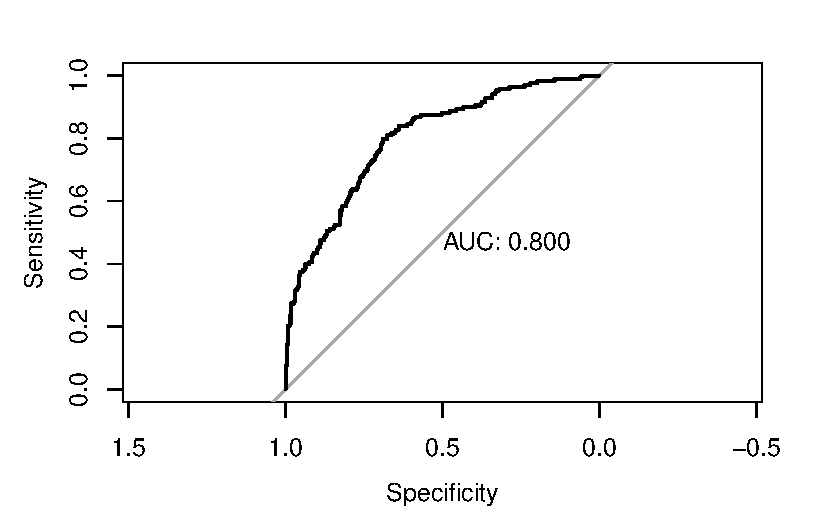
\includegraphics{TP_final_files/figure-pdf/unnamed-chunk-45-1.pdf}

}

\end{figure}

\begin{Shaded}
\begin{Highlighting}[]
\NormalTok{threshold }\OtherTok{\textless{}{-}}\NormalTok{ pROC}\SpecialCharTok{::}\FunctionTok{coords}\NormalTok{(curvaROC, }\StringTok{"best"}\NormalTok{, }\AttributeTok{ret =} \StringTok{"threshold"}\NormalTok{)[}\DecValTok{1}\NormalTok{,]}
\end{Highlighting}
\end{Shaded}

Se obtiene un valor de AUC (área bajo la curva) igual a 0,8, lo cual
habla de un buen clasificador.

Bajo el método de Youden se obtiene un punto de corte óptimo igual a
0.257. Este valor es lejano al punto de corte por defecto: 0,5.

\hypertarget{muxe9tricas-de-capacidad-predictiva}{%
\subsection{Métricas de capacidad
predictiva}\label{muxe9tricas-de-capacidad-predictiva}}

\begin{Shaded}
\begin{Highlighting}[]
\NormalTok{p\_hat }\OtherTok{\textless{}{-}} \FunctionTok{predict}\NormalTok{(logreg\_mod, logreg\_test)}

\NormalTok{observados }\OtherTok{\textless{}{-}}\NormalTok{ logreg\_test }\SpecialCharTok{\%\textgreater{}\%} 
  \FunctionTok{mutate}\NormalTok{(}\AttributeTok{y =} \FunctionTok{if\_else}\NormalTok{(tasa\_grad\_binaria, }\StringTok{"Buena tasa"}\NormalTok{, }\StringTok{"Mala tasa"}\NormalTok{)) }\SpecialCharTok{\%\textgreater{}\%} 
  \FunctionTok{pull}\NormalTok{(y) }\SpecialCharTok{\%\textgreater{}\%} 
  \FunctionTok{factor}\NormalTok{(}\AttributeTok{levels =} \FunctionTok{c}\NormalTok{(}\StringTok{"Mala tasa"}\NormalTok{, }\StringTok{"Buena tasa"}\NormalTok{))}

\NormalTok{predichos }\OtherTok{\textless{}{-}} \FunctionTok{factor}\NormalTok{(}
  \FunctionTok{ifelse}\NormalTok{(p\_hat }\SpecialCharTok{\textgreater{}=}\NormalTok{ threshold, }\StringTok{"Buena tasa"}\NormalTok{, }\StringTok{"Mala tasa"}\NormalTok{), }
  \AttributeTok{levels =} \FunctionTok{c}\NormalTok{(}\StringTok{"Mala tasa"}\NormalTok{, }\StringTok{"Buena tasa"}\NormalTok{)}
\NormalTok{)}
\FunctionTok{confusionMatrix}\NormalTok{(}
  \AttributeTok{data =}\NormalTok{ predichos, }
  \AttributeTok{reference =}\NormalTok{ observados, }
  \AttributeTok{mode =} \StringTok{"everything"}\NormalTok{,}
  \AttributeTok{positive =} \StringTok{"Buena tasa"}
\NormalTok{)}
\end{Highlighting}
\end{Shaded}

\begin{verbatim}
Confusion Matrix and Statistics

            Reference
Prediction   Mala tasa Buena tasa
  Mala tasa        152         44
  Buena tasa         9         27
                                          
               Accuracy : 0.7716          
                 95% CI : (0.7121, 0.8239)
    No Information Rate : 0.694           
    P-Value [Acc > NIR] : 0.005386        
                                          
                  Kappa : 0.3762          
                                          
 Mcnemar's Test P-Value : 3.008e-06       
                                          
            Sensitivity : 0.3803          
            Specificity : 0.9441          
         Pos Pred Value : 0.7500          
         Neg Pred Value : 0.7755          
              Precision : 0.7500          
                 Recall : 0.3803          
                     F1 : 0.5047          
             Prevalence : 0.3060          
         Detection Rate : 0.1164          
   Detection Prevalence : 0.1552          
      Balanced Accuracy : 0.6622          
                                          
       'Positive' Class : Buena tasa      
                                          
\end{verbatim}

\begin{itemize}
\tightlist
\item
  \textbf{Precisión:} El modelo clasifica correctamente al 77\% de las
  universidades del conjunto de prueba según si tienen o no una buena
  tasa de graduación.
\item
  \textbf{Sensibilidad:} Entre las universidades con buena tasa de
  graduación, sólo un 38\% de ellas fueron clasificadas correctamente.
\item
  \textbf{Especificidad:} Entre las universidades con mala tasa de
  graduación, un 94\% fueron clasificadas correctamente.
\item
  \textbf{VPP:} Cuando el modelo predice que una universidad tiene una
  buena tasa de graduación, acierta un 75\% de las veces.
\item
  \textbf{VPN:} Cuando el modelo predice que una universidad tiene una
  mala tasa de graduación, acierta un 78\% de las veces.
\item
  \textbf{F1:} La media armónica entre la sensibilidad y el VPP resulta
  igual a 50\%.
\item
  \textbf{Kappa:} La capacidad predictiva del modelo propuesto es
  aceptable.
\end{itemize}



\end{document}
